%\documentclass[runningheads,a4paper]{lincs}
%\documentclass[sttt]{svjour}
\documentclass{template/openetcs_article}


\usepackage{xspace}
\usepackage{rotating,url,color}
\setcounter{tocdepth}{3}
\usepackage{graphicx}
\usepackage{multirow}
\usepackage[table]{xcolor}
\usepackage{datetime}
\usepackage{moreverb}
\usepackage{fancyvrb}

\urldef{\mailboth}\path|{huang,jp}@informatik.uni-bremen.de|
\newcommand{\keywords}[1]{\par\addvspace\baselineskip
\noindent {\bf Keywords} \enspace\ignorespaces#1}


\DeclareMathSymbol{\B}{\mathalpha}{AMSb}{"42}
\DeclareMathSymbol{\I}{\mathalpha}{AMSb}{"49}
\DeclareMathSymbol{\N}{\mathalpha}{AMSb}{"4E}
\DeclareMathSymbol{\Pwr}{\mathalpha}{AMSb}{"50}
\DeclareMathSymbol{\Q}{\mathalpha}{AMSb}{"51}
\DeclareMathSymbol{\R}{\mathalpha}{AMSb}{"52}
\DeclareMathSymbol{\Z}{\mathalpha}{AMSb}{"5A}
\DeclareMathSymbol{\Sol}{\mathalpha}{AMSb}{"53}

\newcommand{\ebcmd}{\mathsf{EmergencyBrakeCommand}}
\newcommand{\sbcmd}{\mathsf{ServiceBrakeCommand}}

\newcommand{\numreq}{11}
\newcommand{\numsubreq}{29}
\newcommand{\numtc}{34}

\DeclareMathSymbol{\B}{\mathalpha}{AMSb}{"42}
\DeclareMathSymbol{\I}{\mathalpha}{AMSb}{"49}
\DeclareMathSymbol{\N}{\mathalpha}{AMSb}{"4E}
\DeclareMathSymbol{\Pwr}{\mathalpha}{AMSb}{"50}
\DeclareMathSymbol{\Q}{\mathalpha}{AMSb}{"51}
\DeclareMathSymbol{\R}{\mathalpha}{AMSb}{"52}
\DeclareMathSymbol{\Z}{\mathalpha}{AMSb}{"5A}
\DeclareMathSymbol{\Sol}{\mathalpha}{AMSb}{"53}

\newcommand{\obsv}[1]{{\cal O}(#1)}
\newcommand{\ctrl}[1]{{\cal C}(#1)}
\newcommand{\vdot}[1]{\stackrel{.}{#1}}
\newcommand{\power}{\mathbf{P}}

\newcommand{\HS}{{\mathcal H}}

\newcommand{\Interval}{\I}

\newcommand{\ist}{\mbox{{\tt true}}}
\newcommand{\isf}{\mbox{{\tt false}}}
\newcommand{\emptytrace}{\langle~\rangle}
\newcommand{\abegin}{\mathbf{begin}}
\newcommand{\aend}{\mathbf{end}}
\newcommand{\alet}{\mathbf{let}}
\newcommand{\aendlet}{\mathbf{endlet}}
\newcommand{\ain}{\mathbf{in}}
\newcommand{\afor}{\mathbf{for}}
\newcommand{\adownto}{\mathbf{downto}}
\newcommand{\aforall}{\mathbf{foreach}}
\newcommand{\awhile}{\mathbf{while}}
\newcommand{\ado}{\mathbf{do}}
\newcommand{\aenddo}{\mathbf{enddo}}
\newcommand{\acontinue}{\mathbf{continue}}
\newcommand{\aif}{\mathbf{if}}
\newcommand{\athen}{\mathbf{then}}
\newcommand{\aelse}{\mathbf{else}}
\newcommand{\aelseif}{\mathbf{elseif}}
\newcommand{\aendif}{\mathbf{endif}}
\newcommand{\ainout}{\mathbf{inout}}
\newcommand{\aout}{\mathbf{out}}
\newcommand{\aprocedure}{\mathbf{procedure}}
\newcommand{\afunction}{\mathbf{function}}
\newcommand{\abreak}{\mathbf{break}}
\newcommand{\awhere}{\mathbf{where}}
\newcommand{\Sup}[1]{\overline{#1}}
\newcommand{\Inf}[1]{\underline{#1}}

\newcommand{\trl}{/\!/}



\newcommand{\taba}{\hspace*{3mm}{}}
\newcommand{\tabb}{\hspace*{6mm}{}}
\newcommand{\tabc}{\hspace*{9mm}{}}
\newcommand{\tabd}{\hspace*{12mm}{}}
\newcommand{\tabe}{\hspace*{15mm}{}}
\newcommand{\tabf}{\hspace*{18mm}{}}
\newcommand{\tabg}{\hspace*{21mm}{}}
\newcommand{\tabh}{\hspace*{24mm}{}}
\newcommand{\tabi}{\hspace*{27mm}{}}
\newcommand{\tabj}{\hspace*{30mm}{}}
\newcommand{\tabk}{\hspace*{33mm}{}}
\newcommand{\tabl}{\hspace*{68mm}{}}

             
                   
\newcommand{\gca}[1]{F(#1)}
\newcommand{\gcb}[1]{F^*(#1)}
\newcommand{\gclr}{{{L^*\atop\longleftarrow}\atop
                   {\longrightarrow\atop L}}}
\newcommand{\gclrf}{{{F^*\atop\longleftarrow}\atop
                   {\longrightarrow\atop F}}}                   
                   
\newcommand{\gclrj}{{{J^*\atop\longleftarrow}\atop
                   {\longrightarrow\atop J}}}
                                      
\newcommand{\gcaprime}[1]{F'(#1)}
\newcommand{\gcbprime}[1]{F'^*(#1)}
\newcommand{\gclrprime}{{{L'^*\atop\longleftarrow}\atop
                   {\longrightarrow\atop L'}}}  
                   
\newcommand{\gcaone}[1]{G(#1)}
\newcommand{\gcbone}[1]{G*(#1)}
\newcommand{\gclrone}{{{G^*\atop\longleftarrow}\atop
                   {\longrightarrow\atop G}}}                                    
                   
                                                         

\newcommand{\dontshow}[1]{}


\newcommand{\Nat}{{\mathbb N}}
\newcommand{\Real}{{\mathbb R}}

\newcommand{\trans}{\longrightarrow}
\newcommand{\transp}{\longrightarrow_{\power}}
\newcommand{\transl}{\longrightarrow_{L}}
\newcommand{\transg}{\longrightarrow_{G}}
\newcommand{\transcfg}[1]{\stackrel{#1}{\longrightarrow}_{CFG}}
\newcommand{\isdefd}{=_{\mbox{\footnotesize def}}}
\newcommand{\equivdef}{\equiv_{\mbox{\footnotesize def}}}
\newcommand{\mitem}{\mbox{\em M-Item}}
\newcommand{\fun}{\rightarrow}
\newcommand{\pfun}{\not\rightarrow}
\newcommand{\currt}{\hat{t}}

\newcommand{\dom}{\mbox{dom}}
\newcommand{\ran}{\text{ran}}

\newcommand{\sigmaa}{\sigma_A}
\newcommand{\strictimplies}{\stackrel{\bullet}{\Rightarrow}}

\newcommand{\eqc}[2]{[#1;#2]}

\newcommand{\vest}{{V_{\text{\sl est}}}}
\newcommand{\vmax}{{V_{\text{\sl MRSP}}}}
\newcommand{\wout}{\mathsf{W}}
\newcommand{\eout}{\mathsf{EB}}
\newcommand{\areb}{\text{allowRevokeEB}}
\newcommand{\sbia}{\text{SBAvailable}}
\newcommand{\sbz}{\text{sb}_0}
\newcommand{\ticmd}{\text{TICmd}}
\newcommand{\dmicmd}{\text{DMICmd}}

\newcommand{\sob}{\text{speedOnBoard}}
\newcommand{\std}{\text{speedToDriver}}
\newcommand{\pstd}{\text{permittedSpeedToDriver}}
\newcommand{\csmsw}{\text{csmSwitch}}
\newcommand{\sbicmd}{\text{sbiCmd}}
\newcommand{\sbidisplay}{\text{DMIdisplaySBI}}


\newcommand{\dvw}{\text{dV}_{\mathsf{warning}}}
\newcommand{\dvs}{\text{dV}_{\mathsf{sbi}}}
\newcommand{\dve}{\text{dV}_{\mathsf{ebi}}}

\newcommand{\calcw}{\text{dV\_warning(float)}}
\newcommand{\calcs}{\text{dV\_sbi(float)}}
\newcommand{\calce}{\text{dV\_ebi(float)}}
\newcommand{\calcstd}{\text{calc\_speed\_to\_driver()}}
\newcommand{\calcpstd}{\text{calc\_permitted\_speed\_to\_driver()}}
\newcommand{\calcsob}{\text{calc\_speed\_onboard()}}





\newcommand{\qpsc}{\text{qpsc}}
\newcommand{\inpunc}{\text{Input}_{\text{\sl unchanged}}}
\newcommand{\tpsc}{\text{tpsc}}
%\newcommand{\inpch}{\text{Input}_{\text{\sl changed}}}
%\newcommand{\outpun}{\text{Output}_{\text{\sl unchanged}}}


\newcommand{\ta}{\mathbf{A}}
\newcommand{\te}{\mathbf{E}}
\newcommand{\tx}{\mathbf{X}}
\newcommand{\tf}{\mathbf{F}}
\newcommand{\tg}{\mathbf{G}}
\newcommand{\tu}{\mathbf{U}}
\newcommand{\tr}{\mathbf{R}}
\newcommand{\tw}{\mathbf{W}}
\newcommand{\tgt}{\mathbf{G_{\text{\tiny T}}}}

%%%???\newcommand{\ts}{\mathbf{S}}
\newcommand{\ttt}{\mathbf{T}}
\newcommand{\ty}{\mathbf{Y}}
\newcommand{\tz}{\mathbf{Z}}
\newcommand{\too}{\mathbf{O}}

\newcommand{\xbox}{\unskip\nobreak\hfil\penalty50
      \hskip2em\hbox{}\nobreak\hfil$\Box$%
      \parfillskip=0pt \finalhyphendemerits=0 \par}



\usepackage{hyperref}
\graphicspath{{./template/}{.}{./figures/}}

% ===================================================================================
\begin{document}
% ===================================================================================
\frontmatter
\project{openETCS}
%============================
% The document metadata is defined below

%assign a report number here
\reportnum{OETCS/WP4/CSM~--~01/00}

%define your workpackage here
\wp{Work Package 4: ``Verification
\& Validation Strategy''\\
Work Package 7: Tool Chain}


%set a title here
\title{A {SysML} Test Model and Test Suite for the {ETCS} Ceiling Speed Monitor}

%set a subtitle here
\subtitle{Technical report}

%set the date of the report here
\date{2015-10-09}

% define the coverart
\coverart[width=350pt]{openETCS_EUPL.png}
 
%define the type of report
\reporttype{Technical Report}

\author{C\'{e}cile Braunstein \and Wen-ling Huang \and Felix H\"ubner \and Jan
  Peleska \and Uwe Schulze}
\affiliation{University Bremen}
 
\begin{abstract}
This technical report contributes to the openETCS project, work packages 
WP4 -- Verification \& Validation Strategy , and WP7 -- Tool Chain. 
An analysis of the existing ETCS SUBSET-076 system tests for the ETCS onboard 
ceiling speed monitor is presented. Alternative algorithms  with higher test strength are
investigated. The underlying testing technology has been implemented in the RT-Tester
model-based testing tool which has been made available for the openETCS tool chain 
as part of WP7.

Apart from functional and non-functional 
requirements specifications, the published standard of the European Train Control System (ECTS) also contains a collection of system test suites. One of these suites is aimed at testing the Ceiling Speed Monitor (CSM) which is a function of the European Vital Computer (EVC), the main onboard controller of ETCS trains.
In this report we present a detailed comparison of   the CSM test suite specified in the ETCS standard with
tests generated from a CSM test model, using several automated generation strategies.  
The test strength of the suites is evaluated using mutations of a CSM software 
implementation.
It turn out that the test suite specified in the ETCS standard is significantly weaker than any of the suites generated with the model-based approach. The greatest test strength is provided by an equivalence partition testing strategy which has been previously elaborated by the authors. The CSM test model has been elaborated by the authors from the ETCS system requirements. Both the model and the model-based test suites have been made   publicly available.
\keywords{Model-based testing, Equivalence class partition testing, UML/SysML, European Train Control System ETCS, Ceiling Speed Monitoring}
\end{abstract}

\maketitle

\section{Introduction}\label{sec:intro}
% ==========================================================================

\subsection{A Test Model for the ETCS Ceiling Speed Monitor}
In 2011 the {\it model-based testing benchmarks website} www.mbt-benchmarks.org has been 
created with the objective to publish test models that may serve as challenges or benchmarks 
for validating testing theories   and for comparing the capabilities of model-based testing (MBT) tools~\cite{pel2011a}.
In this technical report a novel contribution to this website is presented, a SysML model
of the Ceiling Speed Monitor (CSM) which is part of the European Vital Computer (EVC), the onboard controller of trains conforming to the European Train Control System (ETCS) standard~\cite{ETCS}. In    Section~\ref{sec:ceil} the functional objectives for the CSM are described, and in Section~\ref{sec:modeldesc} the detailed model description is provided. 

The static and behavioural semantics of SysML models have been defined in~\cite{SysML12,uml_2_4} in a semi-formal way, leaving certain ``semantic variation points'' open, so that they can be adjusted according to project-specific requirements. For automated model-based testing, however, a strictly formal semantics is required, so that concrete test data can be calculated from the model's transition relation using constraint solving techniques~\cite{peleska2013ictss}. 
We therefore describe in Section~\ref{sec:transrel} how a formal behavioural semantics is derived for the CSM model and present the associated transition relation in propositional form.

We use state transition systems (STS) for encoding the operational semantics of concrete
modelling formalisms like SysML. STS are widely known from the field of model checking~\cite{clarke_em-etal:1999a}, because their extension into Kripke Structures allows for effective data abstraction techniques. The latter are also applied for equivalence class testing. 
Since state transition systems are a means for semantic representation, testing theories elaborated for STS are applicable for all concrete formalisms whose behavioural semantics can be expressed by STS. In~\cite{d341} it is shown how the semantics of general SysML models and models of a process algebra are encoded as STS. In this technical report we illustrate  how this is achieved for the concrete case of the CSM SysML model.

% ==========================================================================
\subsection{Equivalence Class Partition Testing for the CSM}

The CSM represents a specific test-related challenge: its behaviour depends on actual and allowed speed, and these have conceptually real-valued data domains, so that -- even when   discretising
the input space -- it would be infeasible to exercise all possible combinations of 
inputs on the system under test (SUT). Therefore equivalence class partition (ECP)
 testing strategies have 
to be applied for testing the CSM. While these strategies are well-adopted  in a heuristic manner
in today's industrial test campaigns, practical application of equivalence class testing still lacks 
formal justification of the equivalence classes selected and the sequences of class representatives 
selected as test cases: standard text books used in industry, for example~\cite{spillner2006}, 
only explain the generation of input equivalence class tests for   systems, where the 
SUT reaction to an input class representative is independent on the internal state. Moreover, the systematic calculation of classes from models, as well as their formal justification with respect to
test strength and coverage achieved, is not yet part of today's best practices in industry. 

In contrast to this, formal approaches to equivalence class testing have been studied in the formal methods communities; references to these results  are given in Section~\ref{sec:related}.
In the second main part of this report (Section~\ref{sec:iecpstart}) we therefore describe a recent formal technique for equivalence class testing and its application to testing the CSM. The theoretical 
foundations of this strategy have been published by two of the authors in~\cite{peleska2013ictss}. 
This technical report illustrates its practical application and presents first evaluation details using a 
prototype implementation in an existing MBT tool; the ECP tests are  compared to test results obtained when applying other MBT coverage strategies, such as transition cover or MC/DC coverage (Section~\ref{sec:conventionaltests}). 


% ==========================================================================
\subsection{Fault Models and Completeness Results}


Our ECP strategy
introduces test suites depending on {\it fault models}. This well adopted notion has first been 
introduced in the field of finite state machine (FSM) testing~\cite{petrenko1996}, but is also applicable
to other formal modelling techniques. A fault model consists of a reference model, a conformance relation and a fault domain. The latter is a collection of models whose behaviour may or may not be
consistent to the reference model in the sense of the conformance relation. The test suites generated 
by the ECP strategy described here are {\it complete} with respect to the given fault model: each
system of the fault domain which conforms to the reference model will pass all the generated tests
(this means that the test suite is {\it sound}), and each system in the fault domain that violates the
conformity to the reference model will fail at least  once when tested according to the test suite (the test suite is {\it exhaustive}). 




%%% @todo open proof strategy of the openETCS project





\section{The Ceiling Speed Monitoring Function -- Functional Objectives}
\label{sec:ceil}
% ======================================================================
 
The
European Train Control System ETCS relies on the existence of an onboard controller
in train engines, the \emph{European Vital Computer EVC}. Its functionality and basic architectural features are described in the public ETCS system specification~\cite{ETCS}. 
One functional category of the EVC covers aspects of speed and distance monitoring, to accomplish the  \emph{``\ldots supervision of the speed of the train versus its position, in order to assure that the train remains within the given speed and distance limits.''}~\cite[3.13.1.1]{ETCSSRS-Principles}. Speed and distance monitoring  is decomposed into three sub-functions~\cite[3.13.10.1.2]{ETCSSRS-Principles}, where only one out of these three is active at a point in time:
\begin{enumerate}
\item \emph{Ceiling speed monitoring (CSM)} supervises the observance of the maximal speed allowed according to the current most restrictive speed profile (MRSP). CSM is active while the train does not approach a target (train station, level crossing, or any other   point that must be reached with predefined speed).

\item \emph{Target speed monitoring (TSM)} supervises the observance of the maximal distance-depending  speed, while the train brakes to a target, that is, a location where a given predefined speed (zero or greater zero) must be met.

\item \emph{Release speed monitoring (RSM)} applies when the special target ``end of movement authority (EOA)'' is approached, where the train must come to a stop. RSM supervises the observance of the distance-depending  so-called release speed, when the train approaches the EOA. 
\end{enumerate}

In this technical report we present a complete formal model of the CSM function, with the objective to derive a complete test suite from this model (Section~\ref{sec:iecpstart}).


% ----------------------------------------------------------------------
\section{Model Description}\label{sec:modeldesc}


% .......................................................................
\subsection{Model Availability} 


The ceiling speed monitor has been modelled using the {\it OMG Systems Modeling Language (OMG SysML$^{TM}$)}~\cite{SysML12}. 
The complete   model   is available for download under {\tt http://www.mbt-benchmarks.org}. This is a website dedicated to the publication of test models possessing features that are of general interest for researchers and practitioners in the field of model-based testing (MBT). Moreover, the models may serve as benchmarks for comparing test automation tools with respect to test strength and tool performance. This has been further motivated in~\cite{pel2011a}, where also suggestions for MBT benchmarks are given.
In this section, we give a comprehensive introduction into the formal model.


% .......................................................................
\subsection{Model Components} 

According to the model-based testing approach applied in this report, UML/SysML test models are 
structured into the following basic components.
\begin{enumerate}
\item A package containing the system requirements (Fig.~\ref{fig:req}),
\item A block diagram  (Fig.~\ref{fig:sysif}) identifying 
\begin{itemize}
\item the system under test (SUT),
\item its interface to the operational environment, and
\item the test environment (TE) simulating the ``real'' operational environment during test execution,
\end{itemize}
\item Subordinate block diagrams refining the internal structure of the SUT (Fig.~\ref{fig:sutcomposite}) and the TE, respectively, 
\item State machines associated with the leaf blocks of the structural decompositions of SUT (Fig.~\ref{fig:csmsmtl}) and TE, and
\item Operations associated with blocks. These are referenced by state machines, when evaluating guard conditions or performing actions.
\end{enumerate}



% .......................................................................
\subsection{Model Semantics -- Overview} 

The detailed formal behavioural semantics of SysML test models has been described 
in~\cite[pp.~88]{d341}. This semantics is consistent with the
standards~\cite{uml_2_4,SysML12}, but fixes certain semantic variation points in
 ways that are admissible according to the standards.
In this technical report, however, the semantic details will be explained as far as they are relevant for understanding the model presented here: in the present section, the behavioural   semantics of the CSM model is 
informally explained, and in Section~\ref{sec:transrel}, the formal model semantics is specified by presenting its transition relation. 

The leaf components of the structural model decomposition execute concurrently. For the model under consideration the SUT operates in a sequential manner, but concurrently with its environment. In this test model, the  behaviour of the TE is undetermined; this is interpreted in the way that every possible sequence of input vectors to the SUT would be allowed.  This assumption is reasonable for the example considered here: due to robustness requirements, the ceiling speed monitor must be able to cope with input sequences that may be unreasonable from a physical point of view. TE components are  introduced in situations where only certain types of interactions between operational environment and SUT are possible.  

The model executes according to the {\it run-to-completion} semantics defined 
for state machines in~\cite{uml_2_4}. The model is in a {\it quiescent} (or stable) state, if 
no transition can be executed without an input change. In a quiescent model state, inputs may be changed. If these changes enable a transition, the latter is executed. Since our SUT model is deterministic -- this is typical for safety-relevant applications -- there is no necessity to handle   situations where several transitions are simultaneously enabled. The executed transition, however, may lead to a {\it transient} state, that is, to a state where another transition is enabled. In the run-to-completion semantics this new transition is also executed, and so forth until a quiescent state is reached. Conceptually, the consecutive execution of model transitions is executed in zero time, so that input changes cannot happen until the next quiescent state has been reached. Moreover, models admitting unbounded sequences of transitions between transient states are considered as illegal, and this situation is called a {\it livelock} failure.



% .......................................................................
\subsection{Interfaces}

The interfaces between SUT and its environment are specified in the
internal block diagram displayed in Fig.~\ref{fig:sysif}. All
interfaces are represented as flow ports. The environment writes to
SUT input ports and reads from SUT output ports.

 \begin{figure}
 %%\hspace*{-40mm}
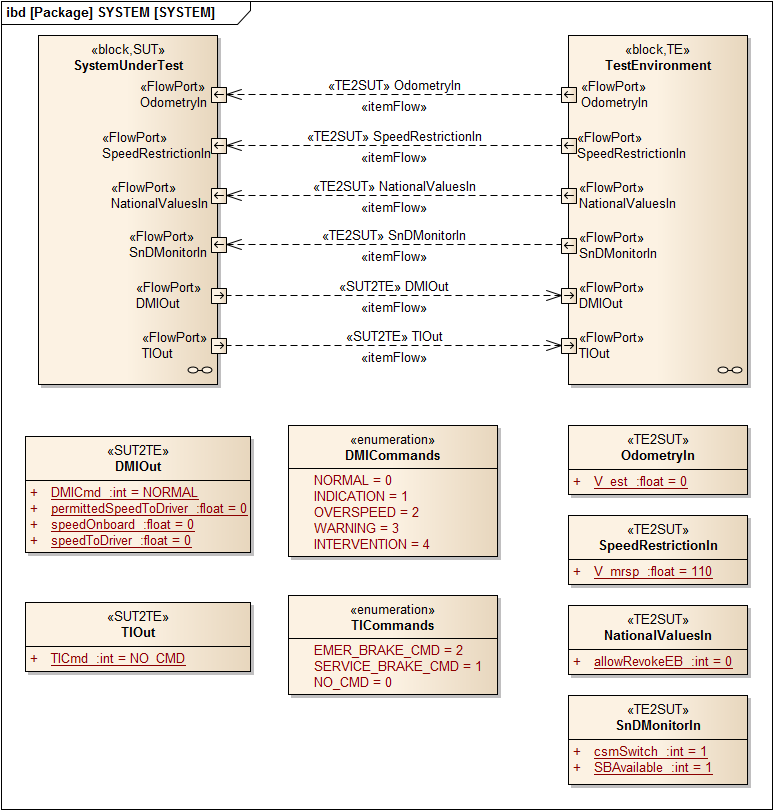
\includegraphics[width=\textwidth]{SYSTEM_INTERFACE.png}
%%\vspace*{-35mm}
\caption{System interface of the ceiling speed monitor.}
 \label{fig:sysif}
 \end{figure}
 
Ceiling speed monitoring is activated and de-activated by the speed and distance monitoring (SnD) coordination function that controls CSM, TSM, and RSM: on input interface {\sf SnDMonitorIn}, variable  $\csmsw$   specifies whether ceiling speed monitoring should be active ($\csmsw=1$) or passive, since target  or release speed monitoring is being performed ($\csmsw = 0$). Furthermore, this interface carries variable $\sbia$ which has value 1, if the train is equipped with a service brake. This brake is then used for slowing down the train if it has exceeded the maximal speed allowed, but not yet reached the threshold for an emergency brake intervention. If $\sbia = 0$, the emergency brake shall be used for slowing down the train in this situation. Input $\sbia$ is to be considered as  a configuration parameter of the train, since it depends on the availability of the service brake hardware. Therefore this value can be freely selected at start-of-test, but must remain constant during test execution.



Input interface {\sf OdometryIn} provides the current speed value
estimated by the odometer equipment in variable $\vest$. Input
interface {\sf SpeedRestrictionIn} provides the current maximal
velocity defined by the most restrictive speed profile in variable
$\vmax$. Input interface {\sf NationalValuesIn} provides a control
flag for the ceiling speed monitor: variable $\text{allowRevokeEB}$ is
1, if after an emergency brake intervention the brake may be
automatically released as soon as the estimated velocity of the train
is again less or equal to the maximal speed allowed. Otherwise
($\text{allowRevokeEB} = 0$) the emergency brakes must only be
released after the train has come to a standstill ($\vest = 0$).
This input parameter is called a ``national value'', because it may change when a
train crosses the boundaries between European countries, due to their local regulations.


Output interface {\sf DMIOut} sends data from the SUT to the driver
machine interface (DMI). It carries five variables. $\dmicmd$ is used
to display the supervision status to the train engine driver: Value
INDICATION may be initially present when CSM is activated, but will be
immediately overridden by one of the values NORMAL, OVERSPEED,
WARNING, or INTERVENTION, as soon as ceiling speed monitoring becomes
active. Value NORMAL is written by the SUT to this variable as long as
the ceiling speed is not violated by the current estimated
speed. Value OVERSPEED has to be set by the CSM as soon as condition
$\vmax < \vest$ becomes true. If the speed increases further (the
detailed conditions are described below), the indication changes from
OVERSPEED to WARNING, and from there to INTERVENTION. The latter value
indicates that either the train is slowed down until it is back in the
normal speed range, or the emergency brake has been triggered to stop
the train.  Furthermore, interface {\sf DMIOut} contains the following 
speed-related variables that are displayed as y/t-diagrams on the DMI.
\begin{itemize}
\item $\std$: the current estimated speed as given by variable $\vest$.
\item $\pstd$: the permitted maximal speed as given by the most 
restrictive speed profile $\vmax$.
\item $\sob$: maximal speed allowed ($\vmax$) as long as the train does not
overspeed.  Otherwise it carries values $\vmax + \delta$, where
$\delta > 0$ specifies the margin from $\vmax$ to service brake
intervention and is calculated as described below.  
\end{itemize}




Output interface {\sf TIout} specifies the train interface from the CSM to the brakes, using 
variable $\text{TICmd}$. If $\text{TICmd} = \text{NO\_CMD}$, both service brakes (if existent) and
emergency brakes are released. If $\text{TICmd} = \text{SERVICE\_BRAKE\_CMD}$, the service brake 
is activated. If $\text{TICmd} = \text{EMER\_BRAKE\_CMD}$, the emergency brake is triggered.



% .......................................................................
\subsection{SUT Attributes and Operations}\label{sec:ops}
The CSM is modelled as an application with sequential behaviour. Therefore the 
SUT block on the top-level interface diagram (Fig.~\ref{fig:sysif})  is refined into another block 
diagram that just carries the SUT, as shown in Fig.~\ref{fig:sutcomposite}.




 \begin{figure}[htbp]
%\hspace*{-50mm}
\centering
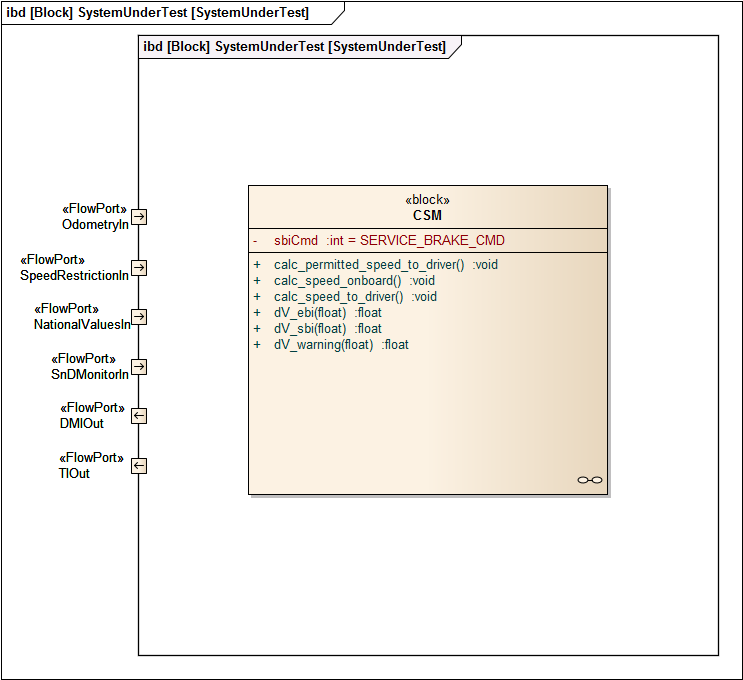
\includegraphics[width=1\textwidth]{SystemUnderTest.png}
%%\vspace*{-35mm}
\caption{Block diagram with CSM (sequential behaviour).}
 \label{fig:sutcomposite}
 \end{figure}



As shown there, the SUT uses a local attribute $\sbicmd$ which 
carries value SERVICE\_BRAKE\_CMD, if the service
brake should be used for slowing down the train to the admissible
speed. If the value EMER\_BRAKE\_CMD is assigned to 
$\sbicmd$, the emergency brake will be triggered in this situation.

Operations $\calcw, \calcs, \calce$ return values that are used to
determine whether a warning should be indicated to the train engine
driver ($\vest > \vmax+\dvw(\vmax)$), a service brake intervention should be
triggered ($\vest > \vmax+\dvs(\vmax)$), or the emergency brake should be
activated ($\vest > \vmax+\dve(\vmax)$).  In each case, the calculation is performed
according to the pattern
\begin{equation}\label{eq:dvcalc}
\text{dV}_x(\vmax) = \left\{
\begin{array}{l}
\min\{\text{dV}_{x\text{min}} + C_x\cdot(\vmax-\text{V}_{x\text{min}}) ,\text{dV}_{x\text{max}} \}  \\\tabh   \text{if}\ \ \vmax > \text{V}_{x\text{min}} \\
\text{dV}_{x\text{min}}  
\\\tabh    \text{if}\ \ \vmax\le  \text{V}_{x\text{min}} \\
\end{array}
\right.
\end{equation}
which has been defined in~\cite[3.13.9.2.3]{ETCSSRS-Principles}. Here $x$ can be replaced by {\sf warning}, {\sf sbi} (SBI = service brake intervention), and {\sf ebi} (EBI = Emergency Brake Intervention), and $C_x$ is defined by 
$$
C_x = \frac{\text{dV}_{x\text{max}} - \text{dV}_{x\text{min}}}{\text{V}_{x\text{max}} - \text{V}_{x\text{min}}}
$$
The following minimal and maximal values apply~\cite[A.3.1]{ETCSSRS-Principles}:

\begin{center}
\bigskip
\begin{tabular}{|l|l|l|}\hline\hline
$\text{dV}_{\mathsf{warning}\text{min}} = 4$ & $\text{dV}_{\mathsf{sbi}\text{min}} = 5.5$ &  $\text{dV}_{\mathsf{ebi}\text{min}} =  7.5$
\\\hline
$\text{dV}_{\mathsf{warning}\text{max}} = 5$ & $\text{dV}_{\mathsf{sbi}\text{max}} = 10$ &  $\text{dV}_{\mathsf{ebi}\text{max}} = 15$
\\\hline\hline
$\text{V}_{\mathsf{warning}\text{min}} = 110$ & $\text{V}_{\mathsf{sbi}\text{min}} = 110$ &  $\text{V}_{\mathsf{ebi}\text{min}} =  110$
\\\hline
$\text{V}_{\mathsf{warning}\text{max}} = 140$ & $\text{V}_{\mathsf{sbi}\text{max}} = 210$ &  $\text{V}_{\mathsf{ebi}\text{max}} = 210$
\\\hline
\hline
\end{tabular}
\end{center}
Inserting these values into Equation~(\ref{eq:dvcalc}) results in
\begin{equation}\label{eq:dvw}
\dvw(\vmax) = \left\{
\begin{array}{lc}
\min\{\frac{1}{3} + \frac{1}{30}\cdot\vmax,5 \}  &    \text{if}\ \ \vmax > 110 \\
4  &  \text{if}\ \ \vmax\le  110 \\
\end{array}
\right.
\end{equation}

\begin{equation}\label{eq:dvsbi}
\dvs(\vmax) = \left\{
\begin{array}{lc}
\min\{0.55+0.045\cdot\vmax,10 \}  &    \text{if}\ \ \vmax > 110 \\
5.5  &  \text{if}\ \ \vmax\le  110 \\
\end{array}
\right.
\end{equation}

\begin{equation}\label{eq:dvwe}
\dve(\vmax) = \left\{
\begin{array}{lc}
\min\{-0.75 + 0.075\cdot\vmax,15 \}  &    \text{if}\ \ \vmax > 110 \\
7.5  &  \text{if}\ \ \vmax\le  110 \\
\end{array}
\right.
\end{equation}

Operations $\calcstd$ and $\calcpstd$ support the display of the current estimated
speed and the maximum speed, respectively, at the driver machine interface by performing assignments to output variables:
\begin{align*}
\std &= \vest\\
\pstd &= \vmax
\end{align*}


Operation $\calcsob$ displays the maximal speed $\vmax$ specified by the most restrictive speed profile in DMI interface variable $\sob$, as long  as the train is not overspeeding. As soon as $\vest > \vmax$, this function calculates the service brake intervention speed and displays it
via  $\sob$, that is,
$$
   \sob = \vmax + \dvs(\vmax)
$$
where $\dvs(\vmax)$ is calculated according to Equation~\ref{eq:dvsbi}.

% .......................................................................
%\newpage
\subsection{Requirements}\label{sec:req}
Figure~\ref{fig:req} shows the requirements reflected by the model.
The requirement labels refer to the sections of the ETCS standard document~\cite{ETCSSRS-Principles}, from where they have been imported into the model. To make   this technical report sufficiently self-contained, we list the requirements applicable to CSM in Table~\ref{tab:req}, and adapt the wording and the cross references to the technical report.

 
In requirement REQ-3.13.10.2.2, the traction cut-off command on the train interface is not explicitly addressed in our model, because it will always be triggered in synchrony with a braking command. We assume the existence of a driver software layer in the EVC that automatically 
triggers traction cut-off  if
\begin{itemize}
\item a traction cut-off interface is implemented for the EVC, and
\item a service brake or emergency brake command is issued.
\end{itemize}

Requirement REQ-3.13.10.2.3 states that national values can only influence the usage of the service brake when in TSM. We will therefore assume that the availability of the service brake and its use for slowing down the train when the emergency braking condition is not yet fulfilled is constant (i.e., $\sbia = 0$ or $\sbia = 1$) during CSM operation.

Requirement REQ-3.13.10.3.3 is described by two tables (see Table~\ref{tab:five} and Table~\ref{tab:six} below), it is then 
decomposed into sub-requirements 
REQ-3.13.10.3.3.t1, \ldots, REQ-3.13.10.3.3.r1, each of them representing one line of these two
tables.

Requirement REQ-3.13.10.3.4 is  represented as a transition table, it
is decomposed into sub-requirements, one for each relevant cells of the
table (see Table~\ref{tab:seven}).  

Requirement REQ-3.13.10.3.7 is ``delegated'' to the surrounding software of the CSM: it is assumed in our model that the input $\vmax$ is always set by the CSM software environment in a way that takes into account the min safe front end of the train.



 \begin{figure}
 \centering
 \hspace*{-20mm}
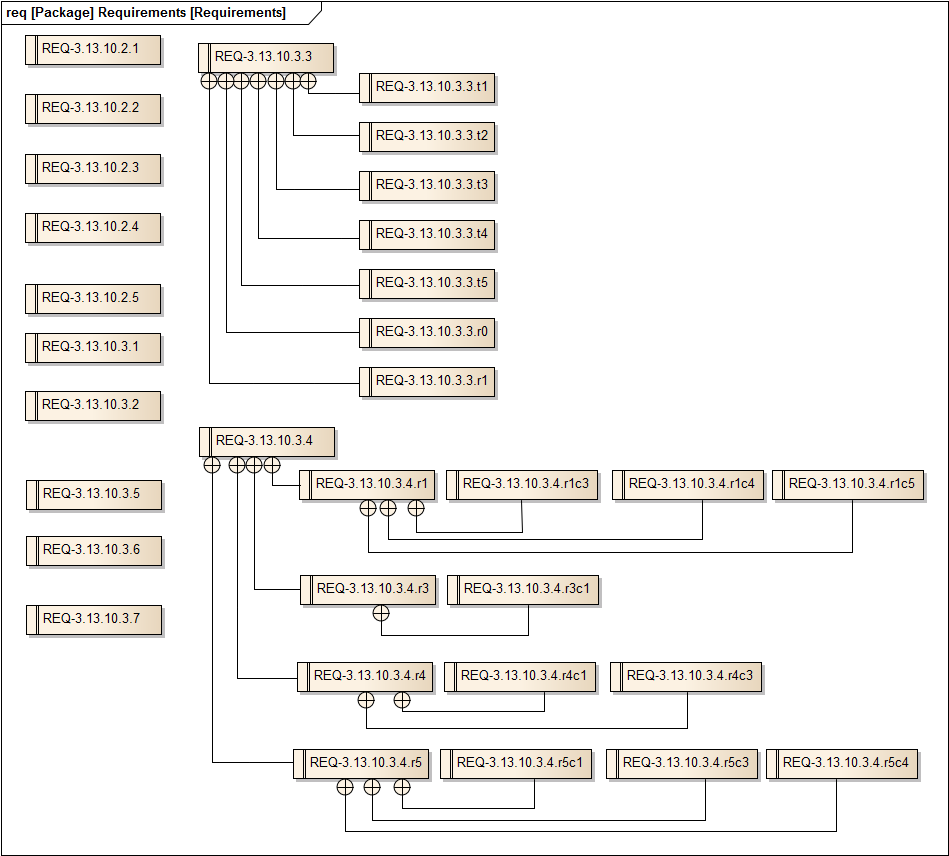
\includegraphics[width=1.3\textwidth]{Requirements.png}
%%\vspace*{-35mm}
\caption{System requirements diagram.}
 \label{fig:req}
 \end{figure}


 \begin{table}[htdp]
\caption{Requirements for the ceiling speed monitoring function.}
%\rule{\textwidth}{1pt}
\begin{center}
\footnotesize
\hspace*{-15mm}
\begin{tabular}{|c|p{130mm}|}
\hline\hline
{\bf id} & {\bf Description}
\\\hline\hline
REQ-3.13.10.2.1 & The train speed indicated to the driver shall be identical to the speed used for the speed monitoring (i.e. the estimated speed $\vest$).
\\\hline
REQ-3.13.10.2.2 & Once a Train Interface command (traction cut-off, service brake or emergency brake) is triggered, the on-board shall apply it until its corresponding revocation condition is met.
\\\hline
REQ-3.13.10.2.3 &
If there is no on-board interface with the service brake or if the use of the service brake command is not allowed by a National Value (only in Target speed monitoring),whenever a service brake command is specified, the emergency brake command shall be triggered instead.
\\\hline
REQ-3.13.10.2.4 &
The emergency brake command, which is triggered instead of the service brake command when an SBI supervision limit is exceeded, shall be revoked according to the requirements specified for the revocation of service brake command, unless the emergency brake command has been also triggered due to an EBI supervision limit. In such case, the condition for revoking the emergency brake command due to EBI supervision limit shall prevail.
\\\hline
REQ-3.13.10.2.5 &
The on-board shall revoke the Intervention status only when no brake command is applied by the speed and distance monitoring function.
\\\hline
%REQ-3.13.10.2.6 &
%In level 2/3: Train trip shall be initiated if the on-board equipment detects that the minimum safe front end has passed the EOA/LOA location.
%\\\hline
%REQ-3.13.10.2.7 &
%In Level 1: Train Trip shall be initiated if the on-board equipment detects that the minimum safe antenna position (calculated by subtracting distance between active Eurobalise antenna and the front end of the train from the min safe front end position) has passed the EOA/LOA location.
%\\\hline
REQ-3.13.10.3.1&
The on-board equipment shall display the permitted speed ($\vmax$).
\\\hline
REQ-3.13.10.3.2 &
When the supervision status is Overspeed, Warning or Intervention, the on-board equipment shall display the SBI speed (i.e. the FLOI speed; FLOI = First Line of Intervention).
\\\hline
REQ-3.13.10.3.3&
The on-board shall compare the estimated speed with the ceiling supervision limits defined in \cite[3.13.9.2]{ETCSSRS-Principles} and shall trigger/revoke commands to the train interface (service brake if implemented or emergency brake) and supervision statuses as described in Table~\ref{tab:five} (from~\cite[Table~5]{ETCSSRS-Principles}) and Table~\ref{tab:six} (from~\cite[Table~6]{ETCSSRS-Principles}).
\\\hline
REQ-3.13.10.3.4&
The on-board equipment shall execute the transitions between the different supervision statuses as described in Table~\ref{tab:seven} (see~\cite[4.6.1]{ETCSSRS-Principles} for details about the symbols). This table takes into account the order of precedence between the supervision statuses and the possible updates of the MRSP while in ceiling speed monitoring (e.g. when a TSR is revoked; TSR = Temporary Speed Restriction).
\\\hline
REQ-3.13.10.3.5&
When the speed and distance monitoring function becomes active and the ceiling speed monitoring is the first one entered, the triggering condition t1 defined in Table~\ref{tab:five} shall be checked in order to determine whether the Normal status applies. If it is not the case, the on-board shall immediately set the supervision status to the relevant value, applying a transition from the Normal status according to Table~\ref{tab:seven}.
\\\hline
REQ-3.13.10.3.6&
The Indication status is not used in ceiling speed monitoring. However, in case the ceiling speed monitoring is entered and the supervision status was previously set to Indication, the on-board equipment shall immediately execute one of the transitions from the Indication status, as described in Table~\ref{tab:seven}.
\\\hline
REQ-3.13.10.3.7&
The locations corresponding to a speed increase of the MRSP shall be supervised by the on-board equipment taking into account the min safe front end of the train.
\\\hline\hline
\end{tabular}
\normalsize
\end{center}
%\rule{\textwidth}{1pt}
\label{tab:req}
\end{table}%
 
\begin{table}[htdp]
\caption{Triggering of Train Interface commands and supervision statuses in ceiling speed monitoring (from~\cite[Table~5]{ETCSSRS-Principles}).}
\begin{center}
\footnotesize
\begin{tabular}{|l|c|l|c|l|}
\hline\hline
{\bf id} & {\bf TC} & {\bf Estimated speed} & {\bf TI} & {\bf SSE} 
\\\hline\hline
REQ-3.13.10.3.3.t1 & t1 & $\vest \le \vmax$ & --- & Normal Status
\\\hline
REQ-3.13.10.3.3.t2 & t2 & $\vest > \vmax$ & --- & Overspeed Status
\\\hline
REQ-3.13.10.3.3.t3 & t3 & $\vest > \vmax + \dvw$ & --- & Warning Status
\\\hline
REQ-3.13.10.3.3.t4 & t4 & $\vest > \vmax + \dvs$ & SB & Intervention Status
\\\hline
REQ-3.13.10.3.3.t5 & t5 & $\vest > \vmax + \dve$ & EB & Intervention Status  
\\\hline\hline
\end{tabular}
\normalsize
\end{center}

TC: trigger condition \newline
TI: command triggered on train interface to brakes \newline
SB: trigger service brake command (if available, otherwise trigger emergency brake)\newline
EB: trigger emergency brake command 
SSE: supervision status entered
\label{tab:five}
\end{table}%


\begin{table}[htdp]
\caption{Revocation of Train Interface commands and supervision statuses in ceiling speed monitoring (from~\cite[Table~6]{ETCSSRS-Principles}).}
\footnotesize
\begin{minipage}{\textwidth}
\begin{center}
\begin{tabular}{|l|c|c|c|p{4cm}|}
\hline\hline
{\bf id} & {\bf RC} & {\bf Estimated Speed} & {\bf TICR} & {\bf SSR}
\\\hline\hline
REQ-3.13.10.3.3.r0 & r0 & Standstill & EB & Intervention Status
\\\hline
REQ-3.13.10.3.3.r1 & r1 & $\vest \le \vmax$ & SB, EB\footnote{Only if $\text{allowRevokeEB} = 1$.} &
Indication Status \newline
Overspeed Status \newline
Warning Status \newline
Intervention Status (if SBI) \newline
Intervention Status (if EB and $\text{allowRevokeEB} = 1$)
\\\hline\hline
\end{tabular}
\end{center}
\end{minipage}
\normalsize

\medskip
RC: revocation condition \newline
TICR: command revoked on train interface to brakes \newline
SSR: supervision status revoked
\label{tab:six}
\end{table}%



\begin{table}[htdp]
\caption{Transitions between supervision statuses in ceiling speed
  monitoring (from~\cite[Table~7]{ETCSSRS-Principles}).}
\begin{center}
\footnotesize
%\begin{tabular}{|p{20mm}|p{20mm}|p{20mm}|p{20mm}|p{20mm}|}
\begin{tabular}{|c|c|c|c|c|}
\hline\hline
Normal Status & $< r1$ & $< r1$ & $< r1$ & $< r0,r1$
\\\hline
 & Indication Status & & & 
 \\\hline
 $t2 >$ & $t2 > $ & Overspeed Status & & 
 \\\hline
 $t3 >$ &  $t3 >$ &  $t3 >$ & Warning Status &
 \\\hline
 $t4,t5 >$ &  $t4,t5 >$ & $t4,t5 >$ & $t4,t5 >$ & Intervention Status
\\\hline\hline
\end{tabular}
\end{center}

\smallskip
 The
  sub-requirements IDs associated with each cell in the transition table
   are of the form  REQ-3.13.10.3.4.rX.cY where X and Y
  are the row and   column indexes, respectively. 
\normalsize
\label{tab:seven}
\end{table}%



% .......................................................................
%\newpage
\subsection{Behavioural Specification}
The behaviour of the ceiling speed monitor is modelled by the hierarchic state machine that is associated with the SUT block of Fig.~\ref{fig:sutcomposite} and displayed in Fig.~\ref{fig:csmsmtl} (top-level state machine) and Fig.~\ref{fig:csmsm} (lower-level state machine associated with composite state {\sf CSM\_ON}.


 \begin{figure}
 \centering
 \hspace*{-15mm}
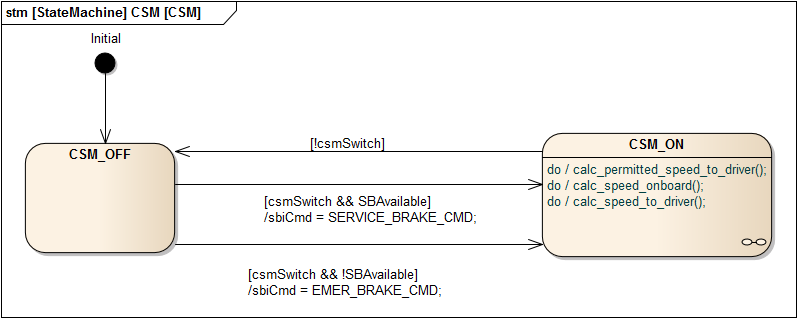
\includegraphics[width=1.2\textwidth]{CSM.png}
%%\vspace*{-35mm}
\caption{Ceiling speed monitoring -- top-level state machine.}
 \label{fig:csmsmtl}
 \end{figure}
 
 
 \begin{figure}
 \centering
\hspace*{-15mm}
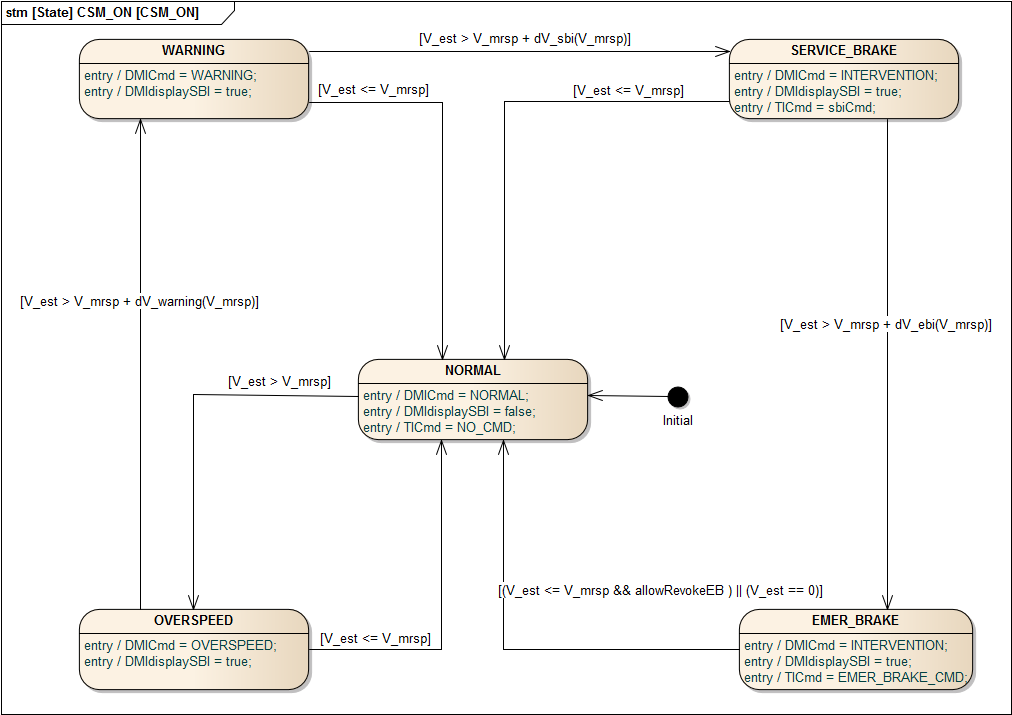
\includegraphics[width=1.2\textwidth]{CSM_ON_NO_FAILURE.png}
%%\vspace*{-35mm}
\caption{Ceiling speed monitoring state machine.}
 \label{fig:csmsm}
 \end{figure}



The top-level state machine controls activation and de-activation of the CSM. As soon as input 
variable $\csmsw$ on interface {\sf SnDMonitorIn} gets value 1, the CSM is activated, and it is de-activated when $\csmsw$ falls back to 0. On activation, the auxiliary variable $\sbicmd$ is set to EMER\_BRAKE\_CMD, if the input variable $\sbia$ carries value 0, indicating that no separate service brake can be used for slowing down the train, so that the emergency brake has to be used for this purpose. Conversely, when $\sbia = 1$, $\sbicmd$ is set to SERVICE\_BRAKE\_CMD. 


While in composite state {\sf CSM\_ON}, do actions are
executed as specified by operations\newline
 $\calcpstd$, $\calcsob$, and   $\calcstd$ 
introduced above. The effect of these
do actions is that variables $\pstd$, $\sob$, and $\std$ 
 are set consistently to the current values depending on $\vest$
and $\vmax$, respectively, as described above. The do-actions are executed whenever all state machine transitions are blocked, and the value of the left-hand side variable of the assignment performed by one of these operations differs from the valuation of the right-hand side expression. As a consequence, the necessary updates of these three output variables are executed in zero time after any input change.

Subordinate state machine {\sf CSM\_ON} specifies the detailed behaviour of the CSM. Its execution starts in basic state {\sf NORMAL}, where the `NORMAL' indication is displayed on the DMI and brakes are released ($\ticmd = \mathsf{NO\_CMD}$). When the speed increases above the maximal speed allowed ($\vest > \vmax$), the state machine transits to basic state {\sf OVERSPEED}, where the `OVERSPEED' indication is displayed to the train engine driver. If the train continues overspeeding until the warning threshold $\vmax + \dvw(\vmax)$ is exceeded, a transition
into the {\sf WARNING} state is performed, accompanied by an indication change on the DMI. Accelerating further until $\vest > \vmax + \dvs(\vmax)$ leads to a transition into basic state {\sf SERVICE\_BRAKE}, where either the service brake or the emergency brake is triggered, depending on the value stored before in variable $\sbicmd$. The DMI display changes to `INTERVENTION'. 

The intervention status is realised by two basic state machine states, {\sf SERVICE\_BRAKE} and
{\sf EMER\_BRAKE}. From {\sf SERVICE\_BRAKE} it is still possible to return to {\sf NORMAL}, as soon as the speed has been decreased below the overspeeding threshold. When the train, however, continues its acceleration until the emergency braking threshold has been exceeded ($\vest > \vmax+\dve(\vmax)$), basic state {\sf EMER\_BRAKE} is entered. From there, a state machine transition to {\sf NORMAL} is only possible if the train comes to a standstill, or if the national regulations (variable $\areb$)
allow to release the brakes as soon as overspeeding has stopped.

Observe that the run-to-completion semantics of state machines also allows for zero-time
 transitions from, for example, {\sf NORMAL} to {\sf EMER\_BRAKE}. If,
 while in basic state {\sf NORMAL},  the inputs change such that
 $\vest > \vmax+\dve(\vmax)$ becomes true\footnote{This would be an
   exceptional behaviour situation, caused, for example, by temporary
   unavailability of odometry data, so that a ``sudden jump'' of
   $\vest$ would be observed by the CSM.}, the state machine
 transition from {\sf NORMAL} to {\sf OVERSPEED} leads to a transient
 model state, because guard condition $\vest > \vmax+\dvw(\vmax)$ is already
 fulfilled, and the state machine transits to {\sf
   WARNING}. Similarly, guards $\vest > \vmax+\dvs(\vmax)$ and $\vest >
 \vmax+\dve(\vmax)$ also evaluate to true, so that the next quiescent state
 is reached in basic state {\sf EMER\_BRAKE}.
  Therefore  REQ-3.13.10.3.4.r5c1  which requires direct transitions from Normal status to Intervention status 
is fulfilled by the {\sf CSM\_ON} state machine: if the guard conditions have the appropriate valuations, the required target states can be reached in zero time, that is, in one observable EVC processing cycle. Analogously, the state machine fulfils requirements 
REQ-3.13.10.3.4.r5c2, REQ-3.13.10.3.4.r5c3, REQ-3.13.10.3.4.r4c1
without needing direct state machine transition arrows between the respective state machine states.


% .......................................................................
\newpage
\subsection{Requirements Tracing} 
SysML provides language elements for relating model elements to requirements, using the {\sf <<satisfy>>} relationship from model elements to requirements symbols in arbitrary SysML diagrams~\cite[Section~16]{SysML12}. Exploiting this language feature supports
\begin{itemize}
\item model validation, and
\item requirements-based testing.
\end{itemize}
In the former case, missing requirements can be detected if they
cannot be linked to structural or behavioural model elements in the
appropriate way. In latter case, execution traces through the model covering a
given structural or behavioural model element represent test cases
contributing to the verification of all requirements related to the
model element under consideration. 

%\begin{table}[htbp]
%\centering
%\includegraphics[height=\textheight]{requirements.pdf}
%\caption{\label{table:req-tracing} Requirements link to the SysML Elements}
%\end{table}


\begin{table}[htbp]
\caption{Requirements links to the SysML Elements}
\scriptsize
\begin{center}
\begin{tabular}{|r|l|l|}
\hline\hline
{\bf No.} & {\bf Requirement} & $\longleftarrow$ {\sf <<satisfy>>}
\\\hline\hline
1 &
REQ-3.13.10.2.1 & {\sf <<Composite State>>} {\sf CSM\_ON}  
\\\hline
2 &
REQ-3.13.10.2.2 & {\sf <<Transition>>} [{\sf EMER\_BRAKE} - {\sf NORMAL}]
\\ & &
{\sf <<Transition>>} [{\sf SERVICE\_BRAKE} - {\sf NORMAL}]
\\\hline
3 &
REQ-3.13.10.2.3 & {\sf <<Transition>>} [{\sf CSM\_OFF} - {\sf CSM\_ON}]
\\ & &
{\sf <<Basic State>>} {\sf SERVICE\_BRAKE}
\\ & &
{\sf <<Constraint>>} constraint\_03 
\\\hline
4 &
REQ-3.13.10.2.4 & {\sf <<Constraint>>} constraint\_02 
\\ & &
{\sf <<Transition>>} [{\sf EMER\_BRAKE} - {\sf NORMAL}]
\\ & &
{\sf <<Constraint>>} constraint\_01 
\\\hline
5 &
REQ-3.13.10.2.5 & {\sf <<Transition>>} [{\sf EMER\_BRAKE} - {\sf NORMAL}]
\\ & &
{\sf <<Transition>>} [{\sf SERVICE\_BRAKE} - {\sf NORMAL}]
\\\hline
6 &
REQ-3.13.10.3.1 & {\sf <<Submachine State>>} {\sf CSM\_ON}
\\\hline
7 &
REQ-3.13.10.3.2 & {\sf <<Basic State>>} {\sf OVERSPEED}  
\\ & &
{\sf <<Basic State>>} {\sf SERVICE\_BRAKE}  
\\ & &
{\sf <<Basic State>>} {\sf WARNING}  
\\ & &
{\sf <<Basic State>>} {\sf EMER\_BRAKE} 
\\\hline
8 &
REQ-3.13.10.3.3.r0 & {\sf <<Transition>>} [{\sf EMER\_BRAKE} - {\sf NORMAL}]
\\\hline
9 &
REQ-3.13.10.3.3.r1 & {\sf <<Transition>>} [{\sf OVERSPEED} - {\sf NORMAL}]
\\ & &
{\sf <<Transition>>} [{\sf SERVICE\_BRAKE} - {\sf NORMAL}]
\\ & &
{\sf <<Transition>>} [{\sf WARNING} - {\sf NORMAL}]
\\ & &
{\sf <<Transition>>} [{\sf EMER\_BRAKE} - {\sf NORMAL}]
\\\hline
10 &
REQ-3.13.10.3.3.t1 & {\sf <<Basic State>>} {\sf NORMAL}  
\\\hline
11 &
REQ-3.13.10.3.3.t2 & {\sf <<Basic State>>} {\sf OVERSPEED}  
\\\hline
12 &
REQ-3.13.10.3.3.t3 & {\sf <<Basic State>>} {\sf WARNING}  
\\\hline
13 &
REQ-3.13.10.3.3.t4 & {\sf <<Basic State>>} {\sf SERVICE\_BRAKE}  
\\\hline
14 &
REQ-3.13.10.3.3.t5 & {\sf <<Basic State>>} {\sf EMER\_BRAKE}  
\\\hline
15 &
REQ-3.13.10.3.4.r1c3 & {\sf <<Transition>>} [{\sf OVERSPEED} - {\sf NORMAL}]
\\\hline
16 &
REQ-3.13.10.3.4.r1c4 & {\sf <<Transition>>} [{\sf WARNING} - {\sf NORMAL}]
\\\hline
17 &
REQ-3.13.10.3.4.r1c5 & {\sf <<Transition>>} [{\sf EMER\_BRAKE} - {\sf NORMAL}]
\\ & &
{\sf <<Transition>>} [{\sf SERVICE\_BRAKE} - {\sf NORMAL}]
\\\hline
18 &
REQ-3.13.10.3.4.r3c1 & {\sf <<Transition>>} [{\sf NORMAL} - {\sf OVERSPEED}]
\\\hline
19 &
REQ-3.13.10.3.4.r4c1 & {\sf <<Constraint>>} constraint\_08 
\\\hline
20 &
REQ-3.13.10.3.4.r4c3 & {\sf <<Transition>>} [{\sf OVERSPEED} - {\sf WARNING}]
\\\hline
21 &
REQ-3.13.10.3.4.r5c1 & {\sf <<Constraint>>} constraint\_10 
\\ & &
{\sf <<Constraint>>} constraint\_09 
\\\hline
22 &
REQ-3.13.10.3.4.r5c3 & {\sf <<Constraint>>} constraint\_12 
\\ & &
{\sf <<Constraint>>} constraint\_11 
\\\hline
23 &
REQ-3.13.10.3.4.r5c4 & {\sf <<Transition>>} [{\sf WARNING} - {\sf SERVICE\_BRAKE}]
\\ & &
{\sf <<Transition>>} [{\sf SERVICE\_BRAKE} - {\sf EMER\_BRAKE}]
\\ & &
{\sf <<Constraint>>} constraint\_13 
\\\hline
24 &
REQ-3.13.10.3.5 & {\sf <<Constraint>>} constraint\_05 
\\ & &
{\sf <<Constraint>>} constraint\_06 
\\ & &
{\sf <<Constraint>>} constraint\_07 
\\ & &
{\sf <<Basic State>>} {\sf NORMAL} 
\\ & &
{\sf <<Constraint>>} constraint\_04 
\\\hline
25 &
REQ-3.13.10.3.6 & {\sf <<Constraint>>} constraint\_05 
\\ & &
{\sf <<Constraint>>} constraint\_06 
\\ & &
{\sf <<Constraint>>} constraint\_07 
\\ & &
{\sf <<Constraint>>} constraint\_04 

\\\hline\hline
\end{tabular}
\end{center}

\hspace*{15mm}
The constraints constraint\_01,\ldots,constraint\_13 are specified in Table~\ref{tab:constraints}.
\normalsize
\label{table:req-tracing} 
\end{table}

Tables \ref{table:req-tracing} associates 
the SysML elements with the requirements they satisfied.  ``Submachine
State'' and  ``Atomic State'' are the top-level and state machine
states, respectively. The ``Constraints" are the LTL formulas used to
relate the most complex requirements to execution traces as explained in the following paragraphs.
 

The complexity of {\sf <<satisfy>>} relations between structural or behavioural model elements depends on the complexity of the requirement and the way each requirement is reflected by the structural and behavioural model. Consider, for example (see Table~\ref{tab:req}), requirement  
\begin{quote}
REQ-3.13.10.2.1: The train speed indicated to the driver shall be identical to the speed used for the speed monitoring (i.e. the estimated speed $\vest$).
\end{quote}
Every model trace where the CSM is activated is suitable for verifying this requirement, because the DMI variable $\std$ is updated by the actual speed $\vest$ via operation $\calcstd$, whenever the ceiling speed monitor is active, that is, in composite state {\sf CSM\_ON}. Therefore 
{\sf CSM\_ON} is linked to REQ-3.13.10.2.1 by the {\sf <<satisfy>>} relation, as expressed
in Table~\ref{table:req-tracing}, row~1. 

 \begin{figure}
 \centering
\hspace*{-10mm}
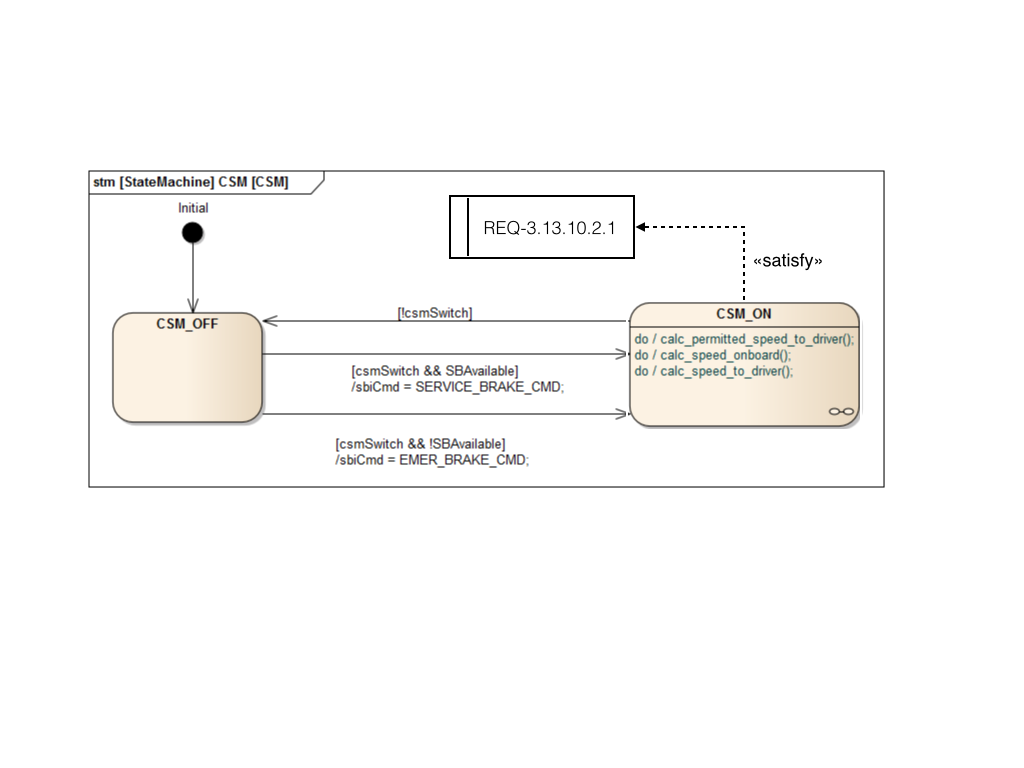
\includegraphics[width=1.2\textwidth]{CSM_ON_SATISFY.png}
\vspace*{-45mm}
\caption{Graphical representation of the {\sf <<satisfy>>} relation in a state machine diagram.}
 \label{fig:satisfy}
 \end{figure}


SysML also allows   to express traceability relationships in a graphical 
way, by drawing arrows from model elements to requirements as shown in Fig.~\ref{fig:satisfy}.
This technique, however, tends to clutter structural and behavioural diagrams as soon as more than a few requirements are involved. Therefore the tabular notation in Table~\ref{table:req-tracing} is preferable and supported by most state-of-the-art SysML modelling tools. 


A more complex case of requirements tracing presents itself if one or more transitions are related to a given requirement. This is the case for the requirement
\begin{quote}
REQ-3.13.10.2.2: Once a Train Interface command (traction cut-off, service brake or emergency brake) is triggered, the on-board shall apply it until its corresponding revocation condition is met.
\end{quote}
As modelled in Fig.~\ref{fig:csmsm}, we have two revocation conditions; one is reflected by the transition from basic state {\sf SERVICE\_BRAKE} to {\sf NORMAL}, the other from {\sf EMER\_BRAKE} to {\sf NORMAL}. Therefore both transitions are related to REQ-3.13.10.2.2, as specified in row~2 of Table~\ref{table:req-tracing}.



%For relating a transition to a requirement, an intermediate constraint is needed, specifying how the transition should be covered in order to check the requirement:
%\begin{itemize}
%\item Constraint keyword `TC' is used to specify that any variable valuation letting the guard condition evaluate to $\ist$ is suitable to verify the requirement.
%\item Constraint keyword `MC/DC' is used to specify that the transition needs to be performed several times, so that its guard condition is covered according to the Modified Condition/Decision Coverage (MC/DC) criterion, in order to verify the requirement.
%\end{itemize}
%The transition is connected to the constraint, and the constraint linked to the requirement by means of the {\sf <<satisfy>>} relationship. In this example, the MC/DC keyword is used in the constraint attached to the state machine transition from {\sf EMER\_BRAKE} to {\sf NORMAL}, because two variants of revocation conditions exist for this case, as specified in Table~\ref{tab:six}: for national value $\areb = 1$, we have to test that the emergency brake is already released when the estimated speed  is again below the maximal speed allowed ($\vest\le\vmax$);
%for $\areb = 0$, we have to test that the brakes are only released after the train has come to a standstill.


In the  most complex case we have to handle situations where requirements are reflected by traces visiting model state {\it vectors}\footnote{A model state vector consists of valuations of  inputs, outputs, and internal model variables, as well as of variable valuations indicating the basic state machine states currently active.} fulfilling certain constraints, and these model state vectors have to be visited by the traces in a specific order. Such a situation is reflected, for example, by 
\begin{quote}
REQ-3.13.10.3.4:
The on-board equipment shall execute the transitions between the different supervision statuses as described in Table~\ref{tab:seven} (see~\cite[4.6.1]{ETCSSRS-Principles} for details about the symbols). This table takes into account the order of precedence between the supervision statuses and the possible updates of the MRSP while in ceiling speed monitoring (e.g. when a TSR is revoked; TSR = Temporary Speed Restriction).
\end{quote}
This requirement   has been decomposed into atomic sub-requirements
REQ-3.13.10.3.4.r1c3, \ldots, REQ-3.13.10.3.4.r5c4, as explained in Section~\ref{sec:req}.
%REQ-3.13.10.3.4.r1c4, REQ-3.13.10.3.4.r1c5, REQ-3.13.10.3.4.r3c1, 
%REQ-3.13.10.3.4.r4c1, REQ-3.13.10.3.4.r4c3, REQ-3.13.10.3.4.r5c1, REQ-3.13.10.3.4.r5c3, REQ-3.13.10.3.4.r5c4, as explained in Section~\ref{sec:req}. 
Some of these sub-requirements are again 
reflected by transitions, as specified in rows 15, 16, 17, 18, and 20 of Table~\ref{table:req-tracing}. Requirement REQ-3.13.10.3.4.r5c1, however, specifies the possibility to directly transit from {\sf NORMAL} to {\sf SERVICE\_BRAKE} or {\sf EMER\_BRAKE}. This cannot be specified by simply linking a behavioural model element to the requirement, because we have avoided to draw direct state machine transitions from {\sf NORMAL} to {\sf SERVICE\_BRAKE} or {\sf EMER\_BRAKE}, since those transitions are implicitly realised by the run-to-completion semantics, as explained above.
Consider, for example, the zero-time transition
{\sf NORMAL} $\trans$ {\sf SERVICE\_BRAKE}. To cover this situation, we need to 
\begin{enumerate}
\item Enter   {\sf NORMAL} in a quiescent model state -- this is specified by 
$$[\mathsf{NORMAL} \wedge \vest \le \vmax]$$
\item Stay there until the speed exceeds $\vmax + \dvs(\vmax)$ but remains less or equal to $\vmax+\dve$.
\end{enumerate}
Formally this is expressed in LTL by 
\[
\begin{array}{l}
 \mathsf{Finally} ([\mathsf{NORMAL}\wedge \vest \le \vmax]  \wedge {}
 \\\tabf
 ([\mathsf{NORMAL}\wedge \vest \le \vmax]
 \\\tabf \ \
 \mathsf{Until}
 \\\tabf\
 [\mathsf{NORMAL}\wedge \vest > \vmax+\dvs(\vmax) \wedge {}
 \\\tabf \  \
 \vest \le \vmax+\dve(\vmax)]))
\end{array}
\]
This is expressed by constraint\_09 linked to REQ-3.13.10.3.4.r5c1 in Table~\ref{table:req-tracing} and specified in Table~\ref{tab:constraints}.
Similarly, covering the zero-time transition {\sf NORMAL} $\trans$ {\sf EMER\_BRAKE} requires a trace satisfying
\[
\begin{array}{l}
 \mathsf{Finally} ([\mathsf{NORMAL}\wedge \vest \le \vmax]  \wedge {}
 \\\tabf
 ([\mathsf{NORMAL}\wedge \vest \le \vmax]
 \\\tabf \ \
 \mathsf{Until}
 \\\tabf\
 [\mathsf{NORMAL}\wedge \vest > \vmax+\dve(\vmax)]))
\end{array}
\]
(this is specified as constraint\_10 in Table~\ref{tab:constraints}).
Similar constraints are specified for REQ-3.13.10.3.4.r4c1, REQ-3.13.10.3.4.r5c3, and 
REQ-3.13.10.3.4.r5c4, and for requirements REQ-3.13.10.3.5 and REQ-3.13.10.3.6.

 




\begin{table}[htdp]
\caption{Constraints related to complex requirements listed in Table~\ref{table:req-tracing}.}
\begin{center}
\scriptsize
\hspace*{-10mm}
\begin{tabular}{|l|p{12cm}|}
\hline\hline
{\sf <<Constraint>>} & {\bf LTL Formula}
\\\hline\hline
constraint\_01 & 
\parbox{120mm}{
\vspace*{1mm}
$\mathbf{Finally} [\mathsf{EMER\_BRAKE} \wedge \neg \sbia \wedge 
         \vest > 0 \wedge \vest \le  \vmax \wedge\neg  \areb]$ 
\vspace*{1mm}         
}
\\\hline
constraint\_02 &  
\parbox{120mm}{
\vspace*{1mm}
$\mathbf{Finally} [\mathsf{SERVICE\_BRAKE} \wedge\neg\sbia \wedge\vest\le\vmax]$
\vspace*{1mm}
}
\\\hline
constraint\_03 &  
\parbox{120mm}{
\vspace*{1mm}
$\mathbf{Finally} [\mathsf{SERVICE\_BRAKE} \wedge\neg\sbia\wedge \vest > \vmax + \dvs(\vmax) \wedge \vest \le \vmax + \dve(\vmax)]$
\vspace*{1mm}
}
\\\hline
constraint\_04 & 
\parbox{120mm}{
\vspace*{1mm}
$\mathbf{Finally} [\mathsf{CSM\_OFF} \wedge \csmsw \wedge \vest > \vmax  \wedge \vest \le \vmax + \dvw(\vmax) ]$
\vspace*{1mm}
} 
\\\hline
constraint\_05 &
\parbox{120mm}{
\vspace*{1mm}
$\mathbf{Finally} [\mathsf{CSM\_OFF} \wedge\csmsw \wedge \vest > \vmax + \dvw(\vmax) \wedge \vest\le\vmax+\dvs(\vmax) ]$
\vspace*{1mm}
}  
\\\hline
constraint\_06 & 
\parbox{120mm}{
\vspace*{1mm}
$\mathbf{Finally} [\mathsf{CSM\_OFF} \wedge\csmsw\wedge \vest > \vmax + \dvs(\vmax) \wedge \vest \le \vmax + \dve(\vmax) ]$
\vspace*{1mm}
} 
\\\hline
constraint\_07 &  
\parbox{120mm}{
\vspace*{1mm}
$\mathbf{Finally} [\mathsf{CSM\_OFF} \wedge\csmsw\wedge \vest > \vmax + \dve(\vmax) ]$
\vspace*{1mm}
}
\\\hline
constraint\_08 &  
\parbox{120mm}{
\vspace*{1mm}
$\mathbf{Finally} ([\mathsf{NORMAL} \wedge \vest\le\vmax] \wedge  
([\mathsf{NORMAL} \wedge  \vest\le\vmax]\ \mathbf{Until}\ [\mathsf{NORMAL} \wedge \vest > \vmax + \dvw(\vmax) \wedge \vest\le\vmax + \dvs(\vmax) ]))$
\vspace*{1mm}
}
\\\hline
constraint\_09 &  
\parbox{120mm}{
\vspace*{1mm}
$\mathbf{Finally} ([\mathsf{NORMAL} \wedge \vest\le\vmax] \wedge  
([\mathsf{NORMAL} \wedge  \vest\le\vmax]\ \mathbf{Until}\ [\mathsf{NORMAL} \wedge \vest > \vmax + \dvs(\vmax) \wedge \vest\le\vmax + \dve(\vmax) ]))$
\vspace*{1mm}
}
\\\hline
constraint\_10 &  
\parbox{120mm}{
\vspace*{1mm}
$\mathbf{Finally} ([\mathsf{NORMAL} \wedge \vest\le\vmax] \wedge  
([\mathsf{NORMAL} \wedge  \vest\le\vmax]\ \mathbf{Until}\ [\mathsf{NORMAL} \wedge \vest > \vmax + \dve(\vmax)]))$
\vspace*{1mm}
}
\\\hline
constraint\_11 &  
\parbox{120mm}{
\vspace*{1mm}
$\mathbf{Finally} ([\mathsf{OVERSPEED} \wedge \vest\le\vmax] \wedge  
([\mathsf{OVERSPEED} \wedge  \vest\le\vmax]\ \mathbf{Until}\ [\mathsf{OVERSPEED} \wedge \vest > \vmax + \dvs(\vmax) \wedge \vest\le\vmax + \dve(\vmax) ]))$
\vspace*{1mm}
}
\\\hline
constraint\_12 &  
\parbox{120mm}{
\vspace*{1mm}
$\mathbf{Finally} ([\mathsf{OVERSPEED} \wedge \vest\le\vmax] \wedge  
([\mathsf{OVERSPEED} \wedge  \vest\le\vmax]\ \mathbf{Until}\ [\mathsf{OVERSPEED} \wedge \vest > \vmax + \dve(\vmax)]))$
\vspace*{1mm}
}
\\\hline
constraint\_13 &  
\parbox{120mm}{
\vspace*{1mm}
$\mathbf{Finally} ([\mathsf{WARNING} \wedge \vest\le\vmax] \wedge  
([\mathsf{WARNING} \wedge  \vest\le\vmax]\ \mathbf{Until}\ [\mathsf{WARNING} \wedge \vest > \vmax + \dve(\vmax)]))$
\vspace*{1mm}
}
\\\hline\hline
\end{tabular}
\normalsize
\end{center}
\label{tab:constraints}
\end{table}%
























\section{Requirements Driven Approach}
\label{sec:req}
\subsection{Formal Requirements Tracing in SysML Models}
\label{sec:formaltrc}
% ============================================================================


%@todo jp: Describe how requirements are formally reflected by sets of computations, and how these sets can be specified by means of LTL safety formulas and revise the 
%following paragraphs


Consider, for example, the zero-time transition
{\sf NORMAL} $\trans$ {\sf SERVICE\_BRAKE}. To cover this situation, we need to 
\begin{enumerate}
\item Enter   {\sf NORMAL} in a quiescent model state -- this is specified by 
$$[\mathsf{NORMAL} \wedge \vest \le \vmax]$$
\item Stay there until the speed exceeds $\vmax + \dvs(\vmax)$ but remains less or equal to $\vmax+\dve$.
\end{enumerate}
Formally this is expressed in LTL by 
\[
\begin{array}{l}
 \mathsf{Finally} ([\mathsf{NORMAL}\wedge \vest \le \vmax]  \wedge {}
 \\\tabf
 ([\mathsf{NORMAL}\wedge \vest \le \vmax]
 \\\tabf \ \
 \mathsf{Until}
 \\\tabf\
 [\mathsf{NORMAL}\wedge \vest > \vmax+\dvs(\vmax) \wedge {}
 \\\tabf \  \
 \vest \le \vmax+\dve(\vmax)]))
\end{array}
\]
This is expressed by constraint\_09 linked to REQ-3.13.10.3.4.r5c1 in Table~\ref{table:req-tracing}.
%% and specified in Table~\ref{tab:constraints}.
Similarly, covering the zero-time transition {\sf NORMAL} $\trans$ {\sf EMER\_BRAKE} requires a trace satisfying
\[
\begin{array}{l}
 \mathsf{Finally} ([\mathsf{NORMAL}\wedge \vest \le \vmax]  \wedge {}
 \\\tabf
 ([\mathsf{NORMAL}\wedge \vest \le \vmax]
 \\\tabf \ \
 \mathsf{Until}
 \\\tabf\
 [\mathsf{NORMAL}\wedge \vest > \vmax+\dve(\vmax)]))
\end{array}
\]
%% (this is specified as constraint\_10 in Table~\ref{tab:constraints}).
Similar constraints are specified for 
REQ-3.13.10.3.4.r1c2,
REQ-3.13.10.3.4.r3c2,
REQ-3.13.10.3.4.r4c1,
REQ-3.13.10.3.4.r4c2,
REQ-3.13.10.3.4.r5c2,
REQ-3.13.10.3.4.r5c3 and 
REQ-3.13.10.3.4.r5c4
as well as for requirements REQ-3.13.10.3.5 and REQ-3.13.10.3.6.


%% \begin{table}
%% \caption{Constraints related to complex requirements listed in Table~\ref{table:req-tracing}.}
%% \begin{center}
%% \scriptsize
%% \hspace*{-10mm}
%% \begin{tabular}{|l|p{12cm}|}
%% \hline\hline
%% {\sf <<Constraint>>} & {\bf LTL Formula}
%% \\\hline\hline
%% constraint\_01 & 
%% \parbox{120mm}{
%% \vspace*{1mm}
%% $\mathbf{Finally} [\mathsf{EMER\_BRAKE} \wedge \neg \sbia \wedge 
%%          \vest > 0 \wedge \vest \le  \vmax \wedge\neg  \areb]$ 
%% \vspace*{1mm}         
%% }
%% \\\hline
%% constraint\_02 &  
%% \parbox{120mm}{
%% \vspace*{1mm}
%% $\mathbf{Finally} [\mathsf{SERVICE\_BRAKE} \wedge\neg\sbia \wedge\vest\le\vmax]$
%% \vspace*{1mm}
%% }
%% \\\hline
%% constraint\_03 &  
%% \parbox{120mm}{
%% \vspace*{1mm}
%% $\mathbf{Finally} [\mathsf{SERVICE\_BRAKE} \wedge\neg\sbia\wedge \vest > \vmax + \dvs(\vmax) \wedge \vest \le \vmax + \dve(\vmax)]$
%% \vspace*{1mm}
%% }
%% \\\hline
%% constraint\_04 & 
%% \parbox{120mm}{
%% \vspace*{1mm}
%% $\mathbf{Finally} [\mathsf{CSM\_OFF} \wedge \csmsw \wedge \vest > \vmax  \wedge \vest \le \vmax + \dvw(\vmax) ]$
%% \vspace*{1mm}
%% } 
%% \\\hline
%% constraint\_05 &
%% \parbox{120mm}{
%% \vspace*{1mm}
%% $\mathbf{Finally} [\mathsf{CSM\_OFF} \wedge\csmsw \wedge \vest > \vmax + \dvw(\vmax) \wedge \vest\le\vmax+\dvs(\vmax) ]$
%% \vspace*{1mm}
%% }  
%% \\\hline
%% constraint\_06 & 
%% \parbox{120mm}{
%% \vspace*{1mm}
%% $\mathbf{Finally} [\mathsf{CSM\_OFF} \wedge\csmsw\wedge \vest > \vmax + \dvs(\vmax) \wedge \vest \le \vmax + \dve(\vmax) ]$
%% \vspace*{1mm}
%% } 
%% \\\hline
%% constraint\_07 &  
%% \parbox{120mm}{
%% \vspace*{1mm}
%% $\mathbf{Finally} [\mathsf{CSM\_OFF} \wedge\csmsw\wedge \vest > \vmax + \dve(\vmax) ]$
%% \vspace*{1mm}
%% }
%% \\\hline
%% constraint\_08 &  
%% \parbox{120mm}{
%% \vspace*{1mm}
%% $\mathbf{Finally} ([\mathsf{NORMAL} \wedge \vest\le\vmax] \wedge  
%% ([\mathsf{NORMAL} \wedge  \vest\le\vmax]\ \mathbf{Until}\ [\mathsf{NORMAL} \wedge \vest > \vmax + \dvw(\vmax) \wedge \vest\le\vmax + \dvs(\vmax) ]))$
%% \vspace*{1mm}
%% }
%% \\\hline
%% constraint\_09 &  
%% \parbox{120mm}{
%% \vspace*{1mm}
%% $\mathbf{Finally} ([\mathsf{NORMAL} \wedge \vest\le\vmax] \wedge  
%% ([\mathsf{NORMAL} \wedge  \vest\le\vmax]\ \mathbf{Until}\ [\mathsf{NORMAL} \wedge \vest > \vmax + \dvs(\vmax) \wedge \vest\le\vmax + \dve(\vmax) ]))$
%% \vspace*{1mm}
%% }
%% \\\hline
%% constraint\_10 &  
%% \parbox{120mm}{
%% \vspace*{1mm}
%% $\mathbf{Finally} ([\mathsf{NORMAL} \wedge \vest\le\vmax] \wedge  
%% ([\mathsf{NORMAL} \wedge  \vest\le\vmax]\ \mathbf{Until}\ [\mathsf{NORMAL} \wedge \vest > \vmax + \dve(\vmax)]))$
%% \vspace*{1mm}
%% }
%% \\\hline
%% constraint\_11 &  
%% \parbox{120mm}{
%% \vspace*{1mm}
%% $\mathbf{Finally} ([\mathsf{OVERSPEED} \wedge \vest\le\vmax] \wedge  
%% ([\mathsf{OVERSPEED} \wedge  \vest\le\vmax]\ \mathbf{Until}\ [\mathsf{OVERSPEED} \wedge \vest > \vmax + \dvs(\vmax) \wedge \vest\le\vmax + \dve(\vmax) ]))$
%% \vspace*{1mm}
%% }
%% \\\hline
%% constraint\_12 &  
%% \parbox{120mm}{
%% \vspace*{1mm}
%% $\mathbf{Finally} ([\mathsf{OVERSPEED} \wedge \vest\le\vmax] \wedge  
%% ([\mathsf{OVERSPEED} \wedge  \vest\le\vmax]\ \mathbf{Until}\ [\mathsf{OVERSPEED} \wedge \vest > \vmax + \dve(\vmax)]))$
%% \vspace*{1mm}
%% }
%% \\\hline
%% constraint\_13 &  
%% \parbox{120mm}{
%% \vspace*{1mm}
%% $\mathbf{Finally} ([\mathsf{WARNING} \wedge \vest\le\vmax] \wedge  
%% ([\mathsf{WARNING} \wedge  \vest\le\vmax]\ \mathbf{Until}\ [\mathsf{WARNING} \wedge \vest > \vmax + \dve(\vmax)]))$
%% \vspace*{1mm}
%% }
%% \\\hline
%% constraint\_14 &  
%% \parbox{120mm}{
%% \vspace*{1mm}
%% $\mathbf{Finally} ([\mathsf{M\_SDMTYPE != CSM} \ \wedge \ 
%% {\sf IndicationStatus}] \mathbf{Until}\ 
%% [\mathsf{M\_SDMTYPE != CSM} \ \wedge \  {\sf IndicationStatus} ] \wedge
%% \mathsf{SUTCommand} \ \wedge \ \vest \leq \vmax ])$
%% \vspace*{1mm}
%% }
%% \\\hline
%% constraint\_15 &  
%% \parbox{120mm}{
%% \vspace*{1mm}
%% $\mathbf{Finally} ([\mathsf{M\_SDMTYPE != CSM} \ \wedge \ 
%% {\sf IndicationStatus}] \mathbf{Until}\ 
%% [\mathsf{M\_SDMTYPE != CSM} \ \wedge \  {\sf IndicationStatus} ] \wedge
%% \mathsf{SUTCommand} \ \wedge \ \vest > \vmax \ \wedge \ \vest \leq \vmax + \dvw(\vmax) ])$
%% \vspace*{1mm}
%% }
%% \\\hline
%% constraint\_16 &  
%% \parbox{120mm}{
%% \vspace*{1mm}
%% $\mathbf{Finally} ([\mathsf{M\_SDMTYPE != CSM} \ \wedge \ 
%% {\sf IndicationStatus}] \mathbf{Until}\ 
%% [\mathsf{M\_SDMTYPE != CSM} \ \wedge \  {\sf IndicationStatus} ] \wedge
%% \mathsf{SUTCommand} \ \wedge \  \vest > \vmax
%% + \dvw(\vmax) \ \wedge \ \vest \leq \vmax + \dvs(\vmax)])$
%% \vspace*{1mm}
%% }
%% \\\hline
%% constraint\_17 &  
%% \parbox{120mm}{
%% \vspace*{1mm}
%% $\mathbf{Finally} ([\mathsf{M\_SDMTYPE != CSM} \ \wedge \ 
%% {\sf IndicationStatus}] \mathbf{Until}\ 
%% [\mathsf{M\_SDMTYPE != CSM} \ \wedge \  {\sf IndicationStatus} ] \wedge
%% \mathsf{SUTCommand} \ \wedge \  \vest > \vmax
%% + \dvs(\vmax) ])$
%% \vspace*{1mm}
%% }
%% \\\hline

%% \hline
%% \end{tabular}
%% \normalsize
%% \end{center}
%% \label{tab:constraints}
%% \end{table}%















% =============================================================================


\subsection{Manually Defined Tests}
\label{sec:manualTest}
The European Railway agency provides a test specification
\cite{ETCS-Subset076} along with the requirements of the EVC.  The
tests aim at verifying the conformity and the functionality of the onboard 
subsystems against the system requirement specification (SRS)
\cite{ETCS}.  The SRS has been decomposed into a set of features such
that a feature groups a set of requirements that can be tested at the
available interfaces. The test cases have been designed to ensure that
a test of a given feature is independent of all other
feature. Moreover tests are only described as a reaction to a given
stimulation at the interface of the feature.

The test specification formalises the test cases
description, each test case is composed of
\begin{itemize}
\item  a unique identifier,
\item  a short description of the target of the test,
\item  a list of covered requirement,
\item an initial state of the test e.g. initial assignment to the
internal test variables,
\item the test  steps:  inputs change and expected outputs, and
\item a final test state e.g. initial assignment to the
internal test variables.
\end{itemize}


Table~\ref{tbl:manualtest} summarizes the available
tests. The second column describes the objective of each test.  The
column ``Covers Requirements'' shows the list of requirements covered
by the tests. We have refined the list provided by the standard. We
first refer to the sub-requirement when needed and secondly, we add
some requirements that are covered by side effect  to be able to
provide more accurate requirement coverage.

The ceiling speed monitoring feature is associated with 8 test cases
in~\cite{ETCS-Subset076}.  They cover the change of the speed
supervision status and the brake commands depending on  the train
speed. We only use seven of them (TC-CSM-[1-7]), the one missing
covers a requirement that we assume, is “delegated” to the surrounding software
of the CSM.
Eight test cases cover the general requirement of the speed and
distance monitoring feature in~\cite{ETCS-Subset076}. Four of those
are test cases outside the scope of the ceiling speed monitoring and
therefore not included in our benchmark.
The four others cover the requirements {\sf REQ-3.13.10.2.3} and
{\sf REQ-3.13.10.2.4} but only in the target speed monitoring section. We
have adapted them to fit into the collection of CSM tests. Moreover,
we grouped them in pairs (TC-GR-[1-2]) . Each pair is dealing with two different ways
of receiving inputs depending on the  ERTMS mode that is not
relevant for testing the CSM function.


\begin{table}
\tabsize
\renewcommand{\arraystretch}{1.2}
\caption{Test cases from the Subset 076}
\label{tbl:manualtest}
\begin{tabular}{lp{.48\textwidth}p{4.9cm}}
\hline\hline
Identifier & Target of the test & Covered Requirements \\
\hline
TC-CSM-1 & 
When the train runs in CSM  and does not exceed the
the permitted speed, no intervention is triggered and the 
{\sf NormalStatus} is displayed.& 
REQ-3.13.10.3.1, REQ-3.13.10.3.3,\newline
REQ-3.13.10.3.5 \\ \hline
TC-CSM-2 & 
When the train runs in CSM and the speed is between the permitted
speed and the Warning limit, no intervention is triggered and the 
{\sf OverspeedStatus} is displayed. Once the train speed is below 
the permitted speed the {\sf NormalStatus} is displayed. & 
REQ-3.13.10.3.1, REQ-3.13.10.3.2,\newline
REQ-3.13.10.3.3, REQ-3.13.10.3.4 \\ \hline
TC-CSM-3 & 
When the train runs in CSM and the speed is between the Warning limit
speed and the SBI supervision limit, no intervention is triggered and the 
{\sf WarningStatus} is displayed. Once the train speed is below 
the permitted speed the {\sf NormalStatus} is displayed. & 
REQ-3.13.10.3.1, REQ-3.13.10.3.2, \newline
REQ-3.13.10.3.3, REQ.3.13.10.3.4.r4 \\ \hline
TC-CSM-4 & 
When the train runs in CSM and the speed is between the SBI
supervision limit and
the EBI supervision limit , the service brake intervention is triggered and the 
{\sf InterventionStatus} is displayed. Once the train speed is below 
the permitted speed the {\sf NormalStatus} is displayed. & 
REQ-3.13.10.2.2, REQ-3.13.10.3.1,\newline
REQ-3.13.10.3.2, REQ-3.13.10.3.3,\newline 
REQ-3.13.10.3.4 \\ \hline
TC-CSM-5 & 
When the train runs in CSM and the speed is greater then 
the EBI supervision limit , the emergency brake intervention is triggered and the 
{\sf InterventionStatus} is displayed. Once the train reaches
standstill the {\sf NormalStatus} is displayed. & 
REQ-3.13.10.2.2, REQ-3.13.10.2.5, \newline
REQ-3.13.10.3.1, REQ-3.13.10.3.2, \newline
REQ-3.13.10.3.3, REQ-3.13.10.3.4 \\ \hline
TC-CSM-6 & 
When entering CSM mode the Indication status is overwritten &
REQ-3.13.10.3.1, REQ-3.13.10.3.3,\newline
REQ-3.13.10.3.4, REQ-3.13.10.3.6 \\ \hline
TC-CSM-7 & 
When the train is between the permitted speed and the Warning limit
the  SBI  supervision limit also referred
as the FLOI (First Line Of Intervention) is 
displayed. Once the train speed is below 
the permitted speed the {\sf NormalStatus} is displayed  & 
REQ-3.13.10.3.1, REQ-3.13.10.3.2,\newline
REQ-3.13.10.3.3, REQ-3.13.10.3.4, \newline
REQ-3.13.10.3.5\\ \hline
TC-GR-1 & 
When the use of service brake is not allowed the emergency brake
command shall be triggered instead. The emergency brake is then revoked
according to the service brake revocation.& 
REQ-3.13.10.2.1, REQ-3.13.10.2.3,\newline
REQ-3.13.10.2.4, REQ-3.13.10.3.3,\newline
REQ-3.13.10.3.4 \\ \hline
TC-GR-2 & 
The use of service brake is not allowed and the train exceeds the EBI
supervision limit, the emergency brake command shall be triggered. 
The emergency brake is then revoked only when the train reaches
standstill.&
REQ-3.13.10.2.1, REQ-3.13.10.2.3,\newline
REQ-3.13.10.2.4, REQ-3.13.10.3.3,\newline
REQ-3.13.10.3.4 \\ 
\hline\hline
\end{tabular}
\normalsize
\end{table}




These 9 test cases has been translated into LTL formula to fit our
experiments platform. This translation is performed by representing
the steps by a sequence of nested until operator.
Let the test sequence be of the following form: $i_0,i_1,o_0,i_2, o_1,o_2$ where
$i_k$ ($o_k$) represents an input (resp. output) assignment to an interface
variables. The associated LTL formula will be in the following form:\\
$$ \mathsf{Finally}( [i_0 \wedge i_1 \wedge o_0] \wedge ([i_0 \wedge i_1 \wedge
o_0] \; \mathsf{Until} \;[i_2 \wedge \mathsf{Finally}([o_1 \wedge o_2]) ) $$
Intuitively the inputs are set and do not change until a new input configuration
is reached and implies new  output values.

\begin{figure}
\begin{Verbatim}[numbers=left]
TC-CSM-2;
 Finally ([currentSpeed > 0 && 
           currentSpeed < V_mrsp &&
           SpeedSupervisionStatus == NormalStatus && 
           displayPermittedSpeed == 1 ]
          &&
          ([currentSpeed > 0 && 
            currentSpeed < V_mrsp &&
            SpeedSupervisionStatus == NormalStatus && 
            displayPermittedSpeed == 1 ]
          Until
          (([currentSpeed > V_mrsp && 
             currentSpeed <= V_mrsp + dV_Waring(V_mrsp)]  && 
             Finally[
                     SpeedSupervisionStatus ==  OverspeedStatus && 
                     displayPermittedSpeed == 1 && 
                     displaySBI == 1 && 
                     ServiceBrakeCommand == 0 ])
              &&
              ([currentSpeed > V_mrsp  && 
                currentSpeed <= V_mrsp + dV_Waring(V_mrsp) ]   
              Until
              ([currentSpeed > 0 && currentSpeed < V_mrsp ] &&
                Finally[SpeedSupervisionStatus == NormalStatus ])))));

\end{Verbatim}
\caption{Example of test case TC-CSM-2 as LTL formula\label{fig:testltlex}}
\end{figure}

Figure \ref{fig:testltlex} shows the LTL formula used to represent the
test case TC-CSM-2. 
\begin{itemize}
\item lines 2-5~: The train is moving within the permitted speed and
the DMI aspects is coherent with the normal status.
\item lines 7-13~: The train stays in the initial configuration until
the speed is greater than permitted speed but below the Warning limit.
\item lines 14-21~: The DMI information changes according to the new
speed.
\item line 23~: The train speed is now back below the permitted.
\item line 24~: The Normal status is now displayed.
\end{itemize}



%%  LocalWords:  EVC EBI WarningStatus InterventionStatus SBI CSM FLOI  REQ
%%  LocalWords:  DMI

\subsection{Extended Manually Defined Tests}
\label{sec:extendedManualTest}
The test specification provided by the European Railway agency (\cite{ETCS-Subset076})
contains test suites for the different ETCS features. The sub-requirements
REQ-3.13.10.3.4.r1c2, REQ-3.13.10.3.4.r3c2, REQ-3.13.10.3.4.r4c2 and REQ-3.13.10.3.4.r5c2
describe a transition from supervision status \emph{Indication} to \emph{Normal}, \emph{Overspeed}, \emph{Warning} and \emph{Intervention}.
Supervision status \emph{Indication} is not used by CSM, but requirement
REQ-3.13.10.3.6 states, that if CSM is ativated with supervision status
being \emph{Indication}, the state changes shall occur as defined in the
sub-requirements above.
The manual test case for REQ-3.13.10.3.6 defined in \cite{ETCS-Subset076}
only covers the state transition from \emph{Indication} to \emph{Normal}.
Therefore the test manual test suite does not cover the sub-requirements
REQ-3.13.10.3.4.r3c2, REQ-3.13.10.3.4.r4c2 and REQ-3.13.10.3.4.r5c2.

Our analysis shows that the sub-requirements REQ-3.13.10.3.4.r5c3 and
REQ-3.13.10.3.4.r5c4 are not covered by the tests defined in \cite{ETCS-Subset076}.
These two sub-requirements define the behaviour of CSM with
supervision status being \emph{Overspeed} and the trigger conditions
require to directly change to \emph{Intervention} (REQ-3.13.10.3.4.r5c3) and
supervision status being \emph{Warning} and the trigger conditions
require to change to \emph{Intervention} (REQ-3.13.10.3.4.r5c4).

To be able to compare the test manually defined suite with automatically
generated test suites presented in \ref{sec:automated_ETCS_test} and the equivalence class testing
approach presented in \ref{sec:ecpt}, additional test procedure have manually been added
to cover the missing requirements\footnote{See table \ref{tbl:extendedmanualtest}}.

\begin{table}
\tabsize
\renewcommand{\arraystretch}{1.2}
\caption{Additional test cases to cover the remaining sub-requirements.}
\label{tbl:extendedmanualtest}
\begin{tabular}{lp{.37\textwidth}p{6.4cm}}
\hline\hline
Identifier & Target of the test & Covered Requirements \\
\hline
TC-CSM-8 & 
When entering CSM mode the Indication status is overwritten &
REQ-3.13.10.3.4.r1c2, REQ-3.13.10.3.4.r3c2,\newline
REQ-3.13.10.3.4.r4c2, REQ-3.13.10.3.4.r5c2,\newline
REQ-3.13.10.3.6 \\ \hline
TC-CSM-9 & 
Switching from \emph{Overspeed} to \emph{Intervention} and \emph{Warning} to \emph{Intervention}&
REQ-3.13.10.3.4.r5c3, REQ-3.13.10.3.4.r5c4 \\
\hline\hline
\end{tabular}
\normalsize
\end{table}

\subsection{Automatically Defined Tests}
\label{sec:automated_ETCS_test}
% ===========================================================
%%@todo jp: check adjustments from uwe
% ===========================================================

The CSM model described in Section~\ref{chap:model} contains
requirement tracing information. Instead of manually translating the
test cases specified for the CSM feature into LTL formulas
\footnote{as described in the previous section \ref{sec:manualTest}},
the requirement tracing information from the model can be
used to automatically generate test procedures covering these
requirements.
%% The tracing information in the test model
%% and the test cases for the feature CSM are both based on the same
%% requirement specification of the CSM feature. In both cases
%% knowledge about the system and understanding of the requirements
%% has been used to interpret the requirement and define tracing
%% information. The difference is where and how the
%% generated tracing information is represented and how it can be used further.
%% When creating the model, the tracing information was directly defined
%% as part of the model in form of SysML satisfy relations.
%% This also allows to review the correctness of this tracing
%% information directly in the test model.
In this section, we describe how the requirement tracing information
defined in the model can be used to automatically generate test
procedures for full requirements coverage from the CSM model.
Note that the test procedures in section \ref{sec:manualTest} also are
automatically generated test procedures providing requirements coverage,
but they have been generated from a manually developed formal test
case specification. The approach presented here uses the requirement
tracing information defined in the model to automatically generate
the formal test case specification and in a second step to
automatically generate the test procedures covering these test cases.
Through this, a test suite is generated in a fully automated way
that covers all requirements represented in the model.

The test generation tool from our experiments platform automatically
generates test cases for different kinds of model coverage strategies
from a test model\footnote{More detailed explanation on the coverage criteria may be found in \cite{D34.1}.}:
\begin{itemize}
\item {\bf Basic Control State Coverage (BCS)}\newline
      This type of behavioural coverage aims at covering each
      basic control state of each state machine at least once.
      No additional objectives are made about concurrent control
      states or accompanying variable valuations when reaching
      the control state under consideration.
\item {\bf Transition Coverage (TR)}\newline
      Transition coverage aims at covering each transition of
      every state machine in the model. Again, no restrictions
      are made regarding variable valuations, control states
      and concurrent transitions to be performed when the one
      under consideration is triggered.
\item {\bf MC/DC Transition Coverage (MCDC)}\newline
      Modified condition/decision (MC/DC) coverage is a variant
      of transition coverage, where non-atomic guard conditions
      are evaluated in a systematic manner.
\item {\bf Hierarchic Transition Coverage (HITR)}\newline
      For a transitions emanating from higher-level control states,
      different underlying basic control states can be active when
      the transition is triggered. Hierarchic transition coverage
      aims at exercising these transitions once for every underlying
      basic control state being active.
\item {\bf Basic Control States Pair Coverage (BCSPAIR)}\newline
      For concurrent state machines pairs of states of two
      different state machines have to be active simultaneously.
      This strategy does not apply to the test model under consideration,
      because it does not contain concurrent state machines.
      \footnote{This coverage criteria does not apply to the CSM
      test model described in chapter \ref{chap:model}, as it
      does not include concurrent state machines.}
%% \item {\bf User Defined LTL Specification (UD)}\newline
%%      For each LTL constraint that is linked to a system component
%%      and that satisfies a requirement, a test case is generated
%%      using the LTL constraint as the test goal.
\end{itemize}

The test model contains requirements together with satisfy relations
linking them to model elements. These requirements are taken directly
from the ETCS specification (\cite{ETCS}).
The requirements 3.13.10.3.3 and 3.13.10.3.4 have been
refined into sub-requirements to allow better tracing to model elements
and to be able to define the requirements coverage in more detail.
%% Therefore, the test model contains \numsubreq{} requirements which can be
%% traced back to the \numreq{} requirements defined for the ceiling speed
%% monitoring feature of ETCS.
Satisfy relations are defined in the model that link transitions,
basic control states or LTL-formulas to requirements.
The test generation tool automatically generates test cases that
cover states, transitions or user defined LTL constraints with
the different test strategies described above.
The satisfy relations defined in the
model are used to determine the set of automatically generated
test cases that satisfy a requirement.
A requirement is covered if the respective set of the automatically
generated test cases (generated from the model) has been covered.

\begin{table}
\caption{Model Derived Requirements Coverage Tests}\label{tbl:derivedtest}
\tabsize
\centering
\begin{tabular}{p{40mm}p{30mm}r}
\hline\hline
Test Procedure Name & Requirements & Number of Test Cases\\
\hline
TP-REQ-3.13.10.2.1 & REQ-3.13.10.2.1 & 1\\
TP-REQ-3.13.10.2.2 & REQ-3.13.10.2.2 & 2\\
TP-REQ-3.13.10.2.3 & REQ-3.13.10.2.3 & 10\\
TP-REQ-3.13.10.2.4 & REQ-3.13.10.2.4 & 3\\
TP-REQ-3.13.10.2.5 & REQ-3.13.10.2.5 & 2\\
TP-REQ-3.13.10.3.1 & REQ-3.13.10.3.1 & 2\\
TP-REQ-3.13.10.3.2 & REQ-3.13.10.3.2 & 18\\
TP-REQ-3.13.10.3.3 & REQ-3.13.10.3.3 & 24\\
TP-REQ-3.13.10.3.4 & REQ-3.13.10.3.4 & 16\\
TP-REQ-3.13.10.3.5 & REQ-3.13.10.3.5 & 6\\
TP-REQ-3.13.10.3.6 & REQ-3.13.10.3.6 & 4\\
\hline\hline
\end{tabular}
\end{table}

For each of the requirements from the ETCS specification, one
test procedure has been generated that covers all automatically generated
test cases that satisfy the requirement (or any of its sub-requirements).
Whether it is possible to completely
cover a requirement in a single test procedure and how well
requirement can be represented in a test model highly depends on
the requirements and on the test model. In this case, we were able
to link all requirements
\footnote{All requirements under consideration that are relevant for ceiling speed monitoring}
from the ETCS specification to
test model elements and to automatically generate a test suite
that provides full requirements coverage.
Table \ref{tbl:derivedtest} also provides the number of test cases that
are covered during the test procedure and that are necessary
to test the requirement. Naturally test cases can occur in multiple
test procedures.



\newcommand{\q}{\textbf{q}}

\section{Improving Tests through Equivalence Class Testing Strategy}\label{sec:ecpt}
\label{sec:ecpt}

 In~\cite{peleska_sttt_2014}, two of the authors have presented a novel complete 
input equivalence class partition (IECP) testing strategy. In \cite{peleska_csm_2014}
this approach has first been applied to the Ceiling Speed Monitor and the analysis of
manually created mutants indicated that this strategy is superior to model derived test cases relying on
structural criteria of the state machine. In \cite{huebner15} the approach was evaluated 
with automatically generated mutants from a Java implementation. Here different refinements of
the strategy were compared and evaluated. For the Ceiling Speed Monitor a mutation score of 100 \%
could be achieved using a combination of equivalence class testing and boundary value tests.  



%@todo: copied from TAP publication, update the following sections for journal
%version

\subsection{Semantic Domain.} 

The novel equivalence class partition testing strategy presented 
in~\cite{peleska_sttt_2014} is applicable to deterministic, livelock-free systems 
with conceptually infinite input domains and finite internal state and output domains.
``Conceptually infinite'' means that the domains are too large to be explicitly 
enumerated for test purposes. This includes physical models with real-valued inputs,
but can also apply to finite but very large data types such as 64 bit integers or
doubles as used in typical programming languages or modelling formalisms. As pointed out 
in~\cite{peleska_sttt_2014,peleska_csm_2014}, this class of systems is quite
significant in the embedded systems domain: typical candidates are controllers 
processing analogue inputs and deriving discrete control decisions from these inputs, such
as thrust reversal controllers in aircrafts, or the speed monitors and airbag controllers described
in this paper.

The strategy has been proven to  be complete on the semantic domain of \emph{Reactive Input Output State Transition Systems (RIOSTS)} ${\cal S} = (S,s_0,R,V,D)$. These systems have state spaces $S$,
initial state $s_0\in S$, and transition relations $R\subseteq S\times S$. Their state spaces
consist of valuation functions $s: V\fun D$, where $V$ is a set of variable symbols and $D$ is 
the union of all variable domains. The variable symbols can be partitioned into $V = I\cup M \cup O$,
where $I$ comprises input variables, $M$ (internal) model variables, and $O$ output variables.
RIOSTS distinguish between \emph{quiescent} states $s\in S_Q$ and \emph{transient} states $s'\in S_T$,
such that $S_Q\cup S_T$ partitions the state space $S$. Transitions from quiescent states only change
input valuations, while internal model variables and output variables remain unchanged. The
resulting post-states may be quiescent or transient. Transitions from transient states always have
uniquely determined quiescent post-states (so we only allow deterministic RIOSTS here), and the associated transitions  leave the inputs
unchanged. This concept represents a natural abstraction of timed formalisms, where 
delay transitions allow for time to pass and inputs to be changed, while discrete
transitions produce output and change internal state, but are executed in zero 
time~\cite[p.~687]{DBLP:books/daglib/0020348}.

By associating atomic propositions $AP$ with free variables in $V$, any RIOSTS can be extended to a 
Kripke Structure~\cite{clarke_em-etal:1999a} 
$K({\cal S}) = (S,s_0,R,V,D,L,AP)$. The labelling function $L:S\fun 2^{AP}$
maps $s\in S$ to the set of all atomic propositions $p\in AP$ that evaluate to $\ist$,
when replacing every free variable $v$ of $p$ by its valuation $s(v)$ in state $s$.

\paragraph{Notation.}
In the exposition below, variable symbols are enumerated with the naming conventions
   $I = \{ x_1,\dots,x_k\}$, $M = \{m_1,\dots, m_p\}$, $O = \{y_1,\dots,y_q\}$. We use   notation
$\vec x = (x_1,\dots,x_k)$  for input variable vectors, and their   valuation in state $s$ is written as $s(\vec x) = (s(x_1),\dots,s(x_k))$. $D_I = D_{x_1}\times\dots\times D_{x_k}$ denotes the Cartesian product of the input variable domains. Tuples $\vec m, \vec y$ and $D_M$ and $D_O$ are defined over model variables and outputs in an analogous way. By $s\oplus\{\vec x \mapsto \vec c\}, \ \vec c \in D_I$ we denote the state $s'$ which coincides with $s$ on all variables from $M\cup O$, but maps the input vector to valuation $s'(\vec x) = \vec c$. 
For $(s_1,s_2)\in R$ we also use the shorter expression $R(s_1,s_2)$.  Restricting a state $s$ to variable symbols from a set $U \subseteq V$ is denoted by $s|_U$. This function has domain $U$ and coincides with $s$ on this domain.

% --------------------------------------------------------------------------
\subsection{Application to Concrete Modelling Formalisms.} 
The test strategy described below is elaborated on the semantic domain of RIOSTS. Every concrete
modelling formalism whose behavioural semantics can be represented by RIOSTS is automatically 
equipped with such a test strategy: the concrete model $M$ is translated into its corresponding RIOSTS ${\cal S}$. Then the test strategy is applied to ${\cal S}$, and this results in a set of test cases, each case represented by a finite sequence of inputs to the SUT. When executing the test cases, 
the transition relation of ${\cal S}$ is used to determine whether the SUT's reactions to these
input sequences are adequate. In this article, concrete models are expressed by SysML state machines,
and these can be associated with RIOSTS semantics which is consistent with the semi-formal specification of state machine behaviour in the UML/SysML standards~\cite{uml_2_4,SysML12}.




% --------------------------------------------------------------------------
\subsection{Equivalence Classes.}
We use the term {\it trace} to denote finite sequences of states, input vectors, or output vectors.
Applying a trace $\iota = \vec c_1\dots\vec c_n$ 
of input vectors $\vec c_i\in D_I$ to an RIOSTS ${\cal S} = (S,s_0,R,V,D)$  residing in some quiescent state
$s\in S$ stimulates a sequence of state transitions, each pair of consecutive states
connected by the transition relation $R$, and with associated  output changes  
as triggered by these inputs. 
Restricting this   sequence to quiescent states, this results in
a trace of states
$\tau = s_1.s_2\dots s_n$ such that $s_i(\vec x) = \vec c_i, i = 1,\dots,n$, and
$s_i(\vec y)$ is the last STS output resulting from application of $\vec c_1\dots\vec c_i$ 
to state $s$.\footnote{Observe that the restriction to quiescent states does not result in a loss
of information. Every transient state has the internal and output variable valuations coinciding with its quiescent pre-state, and its input valuation is identical to that of its quiescent
post-state.} This trace $\tau$ is  denoted by $s/\iota$. The restriction of $s/\iota$ to output variables is denoted by the trace $(s/\iota)|_O$.
Since transient states have unique quiescent post-states, $(s/\iota)|_O$ is a uniquely determined
output trace.
Two quiescent states $s, s'$ are {\it I/O-equivalent}, written $s\sim s'$, 
if every non-empty input trace $\iota$, when applied to $s$ and $s'$, results in the same outputs, that is,  
$(s/\iota)|_O = (s'/\iota)|_O$. Two STS ${\cal S}, {\cal S}'$ with the same input domain are I/O-equivalent, if their initial states 
are I/O-equivalent.
Note that  $s\sim s'$ asserts equivalent I/O-behaviour {\it in the future}, while it still admits that states $s$ and $s'$ show different output valuations, i.e.~$s|_O \neq s'|_O$. 
 

Since I/O-equivalence  $\sim$ is an equivalence relation on quiescent states, 
we can factorise $S_Q$ with respect to  $\sim$.
The \emph{initial input equivalence class partitioning (IECP)} ${\cal I}\subseteq\mathbb{P}(D_I)$ 
associated with $S_Q/_\sim$ is 
the coarsest partitioning of $D_I$ such that for all $\q\in S_Q/_\sim$, $X\in {\cal I}$,
there exists a uniquely determined I/O-equivalence class $ \delta(\q,X)\in S_Q/_\sim$, 
such that
\begin{equation}\label{eq:iecpa}
 \forall s\in \q, \vec c\in X: s/\vec c \in \delta(\q,X)
\end{equation}
and there exists a well-defined output $\omega(\q,X)\in D_O$, such that
\begin{equation}\label{eq:iecpb}
\forall s\in \q, \vec c\in X: (s/\vec c)|_O =  \omega(\q,X)
\end{equation}
It is shown in~\cite{peleska_sttt_2014} that $S_Q/_\sim$ is finite
 if the RIOSTS ${\cal S}$
has finite internal state domains and finite output domains, while the input domains may be infinite.
Moreover,   the coarsest partitioning ${\cal I}$  exists, and it is finite and uniquely determined under these prerequisites.
For these RIOSTS, 
properties (\ref{eq:iecpa}) and (\ref{eq:iecpb}) induce an abstraction    
  to DFSMs   
with state space $S_Q/_\sim$, input alphabet ${\cal I}$, and output alphabet
$D_O$:  (\ref{eq:iecpa})
specifies a well-defined total transition function $\delta : S_Q/_\sim\times {\cal I} \fun S_Q/_\sim$, and (\ref{eq:iecpb}) a well-defined
output function $\omega : S_Q/_\sim\times {\cal I} \fun D_O$.
When partitioning ${\cal I}$ further to a refined IECP $\overline{\cal I}$,
the characteristic properties (\ref{eq:iecpa}),(\ref{eq:iecpb}) are preserved.  

A finite sequence $X_1\dots X_k, X_i\in{\cal I}$   is called an \emph{abstract test case}:
concrete test input vectors $\vec c_i$  can be selected from each $X_i$, and, when applied
to the initial state $s_0$, this selection induces a trace $s_1\dots s_k$ of 
quiescent states, such that
$$
\exists \q_1,\dots,\q_k\in  S_Q/_\sim:\forall i \in \{ 1,\dots,k \}: 
s_i\in \q_i\wedge \q_i = \delta(\q_{i-1},X_i)
$$
The IECP properties imply that the
\emph{expected results} associated with this test case are then specified by the
output trace $\omega(\q_{i-1},X_i), i=1,\dots,k$.


 

In~\cite{peleska_sttt_2014} an algorithm for calculating  $S_Q/_\sim$ and ${\cal I}$ is given.
This algorithm produces propositions over variables from $V$, 
specifying the members of $S_Q/_\sim$ and ${\cal I}$, respectively. Making use of an SMT solver, the algorithm allows for identifying the  reachable I/O-equivalence classes
 $\q \in S_Q/_\sim$. As a consequence, every proposition characterising an abstract test
 case $X_1\dots X_k$  is actually feasible: this means that we can find concrete
traces in ${\cal S}$ such that, after deleting the transient states, the resulting
quiescent state sequence $s_0.s_1\dots s_k$ fulfils $s_i\in\q_i$ for $i = 0,\dots,k$ 
and $s(\vec x)\in X_i$ for $i = 1,\dots,k$.

For the model described in section~\ref{chap:model}, input equivalence
classes are unions of convex subsets of $\mathbb{R}^n$. It should be noted, however, that the
notion of I/O-equivalence and IECPs introduced here is far more general, since arbitrary propositional specifications of I/O-equivalence classes can be handled by the 
underlying theory. The input equivalence classes identified in~\cite[Example~1]{peleska_sttt_2014}, for example, contain members 
$z$ specified by conditions $z\!\! \mod m = n$.




% --------------------------------------------------------------------------
\subsection{Fault Models.}
%Complete black box test strategies are typically defined with respect to a given fault model 
%${\cal F} = ({\cal S},\sqsubseteq,{\cal D})$: ${\cal S}$ is the reference model 
%representing the ideal SUT behaviour. Relation $\sqsubseteq$ is a conformance relation describing
%the acceptable SUT behaviours,  so that an SUT whose behaviour is represented by some  
%${\cal S}'$ shall be accepted if and only if ${\cal S}' \sqsubseteq {\cal S}$.
%The fault domain ${\cal D}$ specifies a set of models that may or may not conform to ${\cal S}$,
%and it is assumed that the true behaviour of the SUT is identical to that of an   ${\cal S}'$
%contained in ${\cal D}$.

For the semantic domain of RIOSTS,
the fault models ${\cal F} = ({\cal S},\sim,{\cal D}({\cal S},m,\overline{{\cal I}}))$ are specified as follows.
The reference models ${\cal S}$ are semantic RIOSTS representations  of models elaborated in concrete formalisms, such that the expected behaviour of the SUT is specified by ${\cal S}$ up to 
I/O-equivalence. We use  I/O-equivalence as conformance relation.


Positive integer $m$ fulfils   
$m\ge n$, where $n$ is the number of I/O-equivalence classes of ${\cal S}$.
IECP $\overline{{\cal I}}$ is a refinement of the initial coarsest IECP ${\cal I}$  associated with ${\cal S}$.
Then the
  members ${\cal S}'$ of the fault domain ${\cal D}({\cal S},m,\overline{{\cal I}})$ 
are RIOSTS specified as follows.
\begin{enumerate}
\item The states of ${\cal S}'$ are defined over the same I/O variable space $ I \cup O$ as defined for the model ${\cal S}$.

\item Initial state $s_0'$ of ${\cal S}'$ coincides with initial state 
$s_0$ of ${\cal S}$ on $I\cup O$. 

\item ${\cal S}'$ generates only finitely many different output values. 

\item ${\cal S}'$ has a well-defined reset operation allowing to re-start the system from its initial state.

\item The number of I/O-equivalence classes of ${\cal S}'$ is less or equal $m$.
 


\item
\label{item:adequacy}  If ${\cal I}$, ${\cal I}'$ are the initial coarsest IECP of  ${\cal S}$, ${\cal S}'$, respectively, 
fulfilling the characteristic properties~(\ref{eq:iecpa}), (\ref{eq:iecpb}), then 
$\overline{{\cal I}}$ fulfils
  the following \emph{adequacy condition}: 
\begin{equation}\label{eq:x2}
\begin{array}{l}
\forall X\in {\cal I}, X'\in {\cal I}':  
\big(X\cap X'\neq\varnothing \Rightarrow
\exists \overline{X}\in \overline{{\cal I}}: \overline{X} \subseteq X\cap X'\big)
\end{array}
\end{equation}


\end{enumerate}



The intuition behind the adequacy condition~\ref{item:adequacy} is as follows. Every possible behaviour of a fault domain member ${\cal S}'$ can be exercised by visiting a state in 
some I/O-equivalence class $\q'$ and applying an input of some IECP member $X'\in {\cal I}'$
to this state. Using the refined IECP $\overline{{\cal I}}$ in the test suite as described below,
ensures that an input from $\overline{X}\subseteq X'\in {\cal I}'$ will be selected when 
${\cal S}'$ resides in $\q'$, so the behaviour associated with $(\q',X')$ will be stimulated in
at least one of the test cases. If,  when in a 
state of $\q'$,  ${\cal S}'$
conforms to the behaviour of ${\cal S}$ for all inputs from $X \setminus X'$, but fails
for inputs from $X\cap X'$, inputs selected from $\overline{X}\subseteq X\cap X'$ will uncover this error.

Conversely, suppose now that
 the reference model  ${\cal S}$ behaves differently, when IECs $X_1, X_2\in {\cal I}$
are applied in some state $\q$. Suppose further that ${\cal S}'$ fails to make this case 
distinction in a corresponding state $\q'$. Then there exists $X'\in {\cal I}'$ such that
 ${\cal S}'$ shows the same behaviour for all $\vec c\in X'$, but $X_1\cap X'\neq \varnothing$
 and $X_2\cap X'\neq \varnothing$, so two different behaviours should be visible according
 to the reference model. Now the adequacy condition guarantees that there exist two IEC
$\overline{X}_1, \overline{X}_2\in \overline{{\cal I}}$, such that 
$\overline{X}_1\subseteq X_1\cap X'$ and 
$\overline{X}_2\subseteq X_2\cap X'$.
 As a consequence, if inputs from every input class 
of $\overline{{\cal I}}$ are exercised, the behavioural differences for inputs from
$X_1\cap X'$ and $X_2\cap X'$ will be revealed. Summarising, the adequacy condition ensures that 
the IECP $\overline{{\cal I}}$ from where input data to the SUT is selected is fine-grained 
enough to stimulate every possibly deviating behaviour of ${\cal S}$ and ${\cal S}'$. These facts
are exploited in the complete test strategy described next.
 
 
 

% ==========================================================================
\subsection{Complete Finite Test Suite.}

The complete DFSM abstraction ${\cal M}$
 of ${\cal S}$ with states $S_Q/_\sim$, input alphabet
 $\overline{{\cal I}}$, transition function and output function
  as characterised in (\ref{eq:iecpa}), (\ref{eq:iecpb}), allows for application of 
finite complete DFSM testing strategies, such as the \emph{W-Method} introduced 
in~\cite{chow:wmethod,vasilevskii1973}. 
The general form of a W-Method test suite is 
\begin{equation}\label{eq:wtestsuite}
{\cal W} = P.\big(\bigcup_{i=0}^{m-n}\overline{\cal I}^i.W\big)
\end{equation}
where $P$ is the state transition cover, $\overline{\cal I}^i$ denotes the input trace segments of length $i$, and $W$ is the characterisation set.  Every test of  ${\cal W}$ consists of a (possibly empty) input trace from $P$, concatenated with an arbitrary input trace of length zero up to $m-n$, and  terminated by an input trace from the characterisation set. 
$P$  is the union of a {\it state cover} $C$ and  a
{\it transition cover} 
$C.\overline{\cal I}$: $C$ contains   the empty trace $\varepsilon$,
 and for any state $\q$ of ${\cal M}$, there exists an input trace in $C$ which, 
 when applied to the initial state, ends at $\q$. The transition cover  
 is defined by 
 $C.\overline{\cal I}=\{\iota.X~|~\iota \in C, X\in \overline{\cal I}\}.$ Summarising, the input sequences of a state transition cover ensure that (1) every state of the reference 
DFSM ${\cal M}$ associated with the reference model ${\cal S}$ is visited, and (2) every transition from every state is exercised.    A characterisation set is a set of input traces distinguishing each pair of states in a minimal DFSM. Using minimisation algorithms such as the one specified in~\cite{gill62}, characterisation sets can be constructed as a by-product of the minimisation process.

The test suite generated according to (\ref{eq:wtestsuite}) is called an 
\emph{abstract test suite}, because its elements are abstract test cases as defined above:
the inputs to be used in each test case are not yet
represented by concrete input vectors $\vec c$, but by input equivalence classes 
$\overline{X}\in \overline{{\cal I}}$. For creating an executable test suite,  inputs
$\vec c\in \overline{X}$ have to be selected for every   
$\overline{X}\in\overline{{\cal I}}$. 

The W-Method is complete for the fault model of all DFSM over the
same input and output alphabet and with at most $m$ states. It is shown in~\cite{peleska_sttt_2014}
that the associated   test suites with concrete inputs $\vec c\in \overline{X}$ are also complete for 
${\cal F} = ({\cal S},\sim,{\cal D}({\cal S},m,\overline{{\cal I}}))$. This completeness 
result is independent on the choice of concrete input data selected from each input 
equivalence class $X\in\overline{\cal I}$.

The fault domain ${\cal D}({\cal S},m,\overline{{\cal I}})$ introduced above
can be extended by increasing $m$ or by refining $\overline{{\cal I}}$. Increasing
$m$ increases the maximal length of input sequences in test cases in a linear way.
This affects the size of the test suite exponentially, 
but allows for fault domain members with 
higher \emph{recurrence diameters} $r$~\cite{biere_linear_2006}: 
this is the length of the longest loop-free path in
a Kripke structure. Erroneous SUT behaviour that only occurs at the end of such a longest loop 
free path may only be detected if the test cases use input sequences that are long enough
to traverse the SUT state up to the length of the recurrence diameter. 

Refining $\overline{{\cal I}}$ increases the size of the IECP, and this size 
increases the number of test cases in a polynomial way. It has to be noted, however,
that uniformly refining all members of $\overline{{\cal I}}$ -- for example, by using 
a sub-paving strategy as it is well known from interval analysis~\cite{jaulin2001} -- increases the size of the IECP exponentially with each new refinement step. 
The resulting fault domain contains members ${\cal S}'$ 
possessing narrower \emph{trapdoors}: these
are refined input guard conditions $g\wedge \delta$ applicable in certain ${\cal S}'$-states,
where  ${\cal S}'$ should behave uniformly for all inputs satisfying $g$. 
The true behaviour of ${\cal S}'$, however, 
conforms to the expected behaviour modelled by ${\cal S}$ only for inputs
fulfilling $g\wedge \neg\delta$, while   erroneous behaviour is revealed for inputs 
satisfying $g\wedge \delta$.

\subsection{Refinement and Randomisation of Equivalence Partition Tests}\label{sec:ecpt:refinement}
%\subsection{Randomisation of Equivalence Partition Tests}\label{sec:randomisation}

As we have seen above, the fault domain ${\cal D}({\cal S},m,\overline{{\cal I}})$ can be enlarged
via $m$ or $\overline{{\cal I}}$. As a drawback this seriously affects the size of the
resulting complete test suite ${\cal W}$. Therefore a refinement of the input equivalence 
class partitioning $\overline{{\cal I}}$ should be used which effectively increases the resulting 
test suites ability to uncover faults. In \cite{huebner15} two refinement heuristics were investigated and it could be
shown that these heuristics are able to improve the test strength of the resulting test suite.
Basically these two improvements work as follows:

\begin{enumerate}
  \item An input partitioning $\overline{\cal I}$ is used. $\overline{\cal I}$ is a refinement of the initial coarsest IECP and
reflects all case distinctions visible in guard conditions.
\item Additionally all boundary value conditions can be used in order to generate boundary
value tests of the original equivalence classes
\footnote{This can be done by adding extra constraints defining the
  boundaries of the original equivalence classes. As an example
  consider the guard condition $x\leq n$ restricting the input
  variable $x$ in input equivalence class $\overline{X}\in
  \overline{\cal I}$ to values less or equal $n$. In this case the
  additional constraint $\gamma$ defined as $x=n$ yields two new
  equivalence classes $\overline{X}_\gamma\subset\overline{X} $ and
  $\overline{X}_{\neg\gamma}\subset\overline{X}$ with
  $\overline{X}_{\gamma}\cap
  \overline{X}_{\neg\gamma}=\emptyset$. $\overline{X}_{\gamma}$ is the
  set of input vectors $\vec c_{\overline{X}_\gamma}$ that fulfill
  $x=n$ and thus are the boundaries of the original equivalence class
  $\overline{X}$ containing all input vectors, where $x<n$ or $x=n$.}.
\end{enumerate}


% As we have seen above, enlarging the fault domain 
% ${\cal D}({\cal S},m,\overline{{\cal I}})$ via $m$ or $\overline{{\cal I}}$ 
% seriously affects the size of the
% resulting complete test suite ${\cal W}$. 

In \cite{huebner15} another improvement of the equivalence class approach has been
presented. This strategy 
% We therefore investigate an alternative approach
% in this paper that 
aims at increasing the test strength of ${\cal W}$
   for SUTs ${\cal S}''$ whose
true behaviour is reflected by RIOSTS   {\it outside} 
${\cal D}({\cal S},m,\overline{{\cal I}})$. For obvious reasons it is assumed that these 
SUTs still fulfil  the RIOSTS 
compatibility requirements 1 -- 4 of the fault domain definition. This means that
${\cal S}''$ may have more than $m$ I/O-equivalence classes and may need an IECP
that is more fine-grained than $\overline{{\cal I}}$, but it is still assumed that 
${\cal S}''$ is an RIOSTS using the same I/O variables and possessing the same visible
initial state and fulfilling a reset condition.

To this end, we observe that the completeness property of the test suites introduced 
above does not depend on the concrete values selected from each input equivalence 
class $\overline{X}\in \overline{{\cal I}}$. For members ${\cal S}'\in {\cal D}({\cal S},m,\overline{{\cal I}})$ it would suffice to fix one input vector 
$\vec c_{\overline{X}}$ for every
$\overline{X}\in \overline{{\cal I}}$. Alternatively, we could also choose different members at random,
each time an input from some class $\overline{X}$ 
is required according to the abstract test suite
definition.
% and decide at random whether to choose internal or boundary 
% values from   $\overline{X}$.
While this alternative would not affect the suite's completeness property
when applied against members of ${\cal D}({\cal S},m,\overline{{\cal I}})$,
it favourably affects the test strength against RIOSTS outside 
${\cal D}({\cal S},m,\overline{{\cal I}})$: the chances for uncovering trapdoors
are obviously increased. This approach results in an 
\emph{adaptive random testing strategy}, where the selection of input data is no longer 
performed uniformly over the complete input domain, but selectively for each input equivalence
class $\overline{X}\in \overline{{\cal I}}$. Moreover, the random values from such 
an $\overline{X}$ are only applied when an $\overline{X}$-input is required according to the 
abstract test suite constructed from Equation~(\ref{eq:wtestsuite}). The experimental results in
\cite{huebner15} indicate, that the randomisation of the input selection is able to improve the 
mutation score for erroneous implementations that are {\it outside} the fault domain without increasing
the size of the resulting test suite and without nullifying the completeness result for 
implementations inside the fault domain.
  


% Technically the randomisation is implemented by running an SMT solver
% repeatedly to find concrete values of every input equivalence class
% $\overline{X}\in \overline{{\cal I}}$. The abstract test suite constructed from
% Equation~(\ref{eq:wtestsuite}) is a sequence on input equivalence classes. According to
% our equivalence class construction \cite{peleska_sttt_2014},
% an input equivalence class $\overline{X}\in \overline{{\cal I}}$ is defined by
% a proposition\footnote{The proposition is
% guaranteed to have a solution, since it describes an input equivalence class,
% which has at least one member and thus at least one assignment that fulfills the
% proposition.}  $g_{\overline{X}}$, containing solely variables in $I$.
% Using an SMT solver to solve  $g_{\overline{X}}$ results in a concrete input
% vector $\vec c \in{\overline{X}}$. Rerunning the solver for the same
% $\overline{X}$ and prohibiting existing solutions $c_1, \ldots, c_{n-1}$
% with a refined constraint
% $g_{\overline{X}}\land\overset{n-1}{\underset{i=1}{\bigwedge}}\neg c_i$ will
% result in a new solution $c_n$, i.e.
% a new concrete input $c_n\in \overline{X}$ of the input equivalence class. 
% The negation of existing solution yields an exponential growth of the runtime of
% the SMT solver in the worst case. Therefore two other heuristics were
% implemented:\\
% (a) the internal heuristics of the SAT solver have been randomized to get a
% ``random'' solution of $g_{\overline{X}}$. 
% (b)
% Interval analysis can be used to find a subpaving, that is an inner approximation of $g_{\overline{X}}$. From
% this subpaving random elements can be selected using a random number generator.
% As another runtime optimization the input selection can be parallelized. Once
% the input equivalence class partitioning $\overline{\cal I}$ is  available, candidates
% from every input equivalence class
% $\overline{X}$ can be calculated separately and in parallel, to find as many
% different concrete values as needed. 
% % The construction of the test oracles, i.e.
% % the expected outputs resulting from the execution of an input sequence from the
% % test suite ${\cal W}$ can be calculated from the abstract test suite and is
% % independent of the concrete inputs. 

% It has to be noted, however, that the complete test suite generated according to
% (\ref{eq:wtestsuite}) will not guarantee that every pair $(\q,\overline{X})$ with $\q\in S/_\sim$ and
% $\overline{X}\in\overline{\cal I}$ will be exercised the same number of times. Therefore we add
% test cases to ensure a minimal number $a$ each $(\q,\overline{X})$ is exercised, each time with 
% a new random selection $\vec c\in \overline{X}$. For these additional test cases we just repeat
% suitable cases from ${\cal W}$. If $p$ estimates the probability to detect a trapdoor when
% selecting a random value in $(\q,\overline{X})$, then the probability to uncover this during the
% randomised test suite is $1 - (1 - p)^a$.

% ----------------------------------------------------------------------
\section{Experimental Results}\label{chap:results}

This section compares the generated test suites presented in the previous
chapters in terms of requirements coverage, model coverage and test strength.
Test suites with the same requirements coverage can provide different model coverage.
Higher model coverage indicates higher test strength, but test suites with
the same model coverage can still be of different test strength. Mutations
of the System Under Test are used to measure the test strength of the
generated test suites.

We will refer to the different test suites as
\emph{Test Suite A} (test procedures generated automatically from manually
defined test case specifications)
\footnote{explained in section \ref{sec:manualTest}.},
\emph{Test Suite B} (test procedures generated automatically from manually
defined test case specifications including additional test cases to cover all remaining sub-requirements)
\footnote{explained in section \ref{sec:extendedManualTest}.},
\emph{Test Suite C} (test procedures generated automatically from
automatically generated test case specifications)
\footnote{explained in section \ref{sec:automated_ETCS_test}.}
and \emph{Test Suite D}
(test procedures generated using the \emph{Equivalence Class Testing}
strategy).
\footnote{as explained in section~\ref{sec:ecpt} including the refinements and randomisation as presented in section~\ref{sec:ecpt:refinement}.}
Section \ref{sec:coverage} presents the requirement
and model coverage results and section \ref{sec:mutations} compares the
test strength of the different test suites.

% .......................................................................
% .......................................................................
\subsection{Requirements and Model Coverage}\label{sec:coverage}

\begin{table}
\caption{Requirements Coverage and Model Coverage Overview.}\label{tbl:coverage}
\centering
% ============================================================================
% @done: Uwe: Put the new numbers/Check the numbers consistency
% ============================================================================

\footnotesize
\begin{tabular}{p{38mm}p{20mm}p{20mm}p{20mm}p{20mm}}
\hline\hline
&
{\bf Manually Defined Tests (A)} &
{\bf Extended Manual Tests (B)} &
{\bf Automatically Defined Tests (C)} &
{\bf Equivalence Class\newline Testing (D)}
\\\hline
{\bf Requirements Coverage}\newline(ETCS specification)&
24 of \numsubreq\newline(82,76\%)&
\numsubreq{} of \numsubreq\newline(100\%)&
\numsubreq{} of \numsubreq\newline(100\%)&
\numsubreq{} of \numsubreq\newline(100\%)
\\\hline
{\bf Test Cases}&
9&
11&
45&
5524
\\\hline
{\bf Model Coverage}\newline
States&
9 of 9\newline(100\%)&
9 of 9\newline(100\%)&
9 of 9\newline(100\%)&
9 of 9\newline(100\%)
\\\hline
{\bf Model Coverage}\newline
Transitions&
10 of 10\newline(100\%)&
10 of 10\newline(100\%)&
10 of 10\newline(100\%)&
10 of 10\newline(90\%)
\\\hline
{\bf Model Coverage}\newline
MCDC&
8 of 10\newline(80\%)&
8 of 10\newline(80\%)&
10 of 10\newline(100\%)&
10 of 10\newline(100\%)
\\\hline

{\bf Model Coverage}\newline
HITR&
1 of 5\newline(20\%)&
3 of 5\newline(60\%)&
5 of 5\newline(100\%)&
5 of 5\newline(100\%)
\\\hline\hline
\end{tabular}
\normalsize
\label{tab:rtt:advanced}
\end{table}%

% --------------------------------------------------------------------------
%Paragraphs describing requirements coverage:

In Table \ref{tab:rtt:advanced} we compare the requirements and the model coverage
of the test suites. Although all test suites cover all states and transitions of
the model at least once, \emph{Test Suite A} does not cover all requirements
completely (not all sub-requirements are covered).
Each of the other three test suites covers all requirements
of ETCS defined in \cite{ETCS-Subset076} including the sub-requirements from our
analysis.

Though \emph{Test Suite B} does cover all requirements, it does not cover all
test cases that are automatically generated from the test model.
Fewer combinations for guard conditions and high level transitions are executed
with this test suite.

The fully automatically generated \emph{Test Suite C} provides full requirements
coverage which is expected, as this is the goal of the test suite.
It also provides full model coverage which is an indication for testable
requirements, a model that has been developed for testing purposes and for
carefully defined satisfy relations from model elements to requirements.

The test traces that are generated for \emph{Test Suite D} have been evaluated on
the test model as well and through this, a test case coverage and requirements coverage
has been calculated using the tracing information from the test model.
\emph{Test Suite C} and \emph{Test Suite D} both achieve the same requirements
and model coverage, but \emph{Test Suite D} uses more test cases to reach this
coverage. In the following section, we will evaluate if the additional test cases
result in an increased test strength of this test suite.


% .......................................................................
% .......................................................................
\subsection{Test Strength Comparison}\label{sec:mutations}

\subsubsection*{Experimental Setup.}

The strength of a test suite is the ability to detect real faults. 
\cite{just_are_2014} shows that mutants are a valid substitute for real faults
when comparing generated test suites. Mutants are modifications of the SUT with (automatically) seeded single faults. 
Mutants in large numbers can be generated 
by mutation operators, which apply slight syntactical changes
to the original code.
To compare the test strength of the generated test suites we measured the mutation score of 
each test suite. The mutation score is the ratio of mutants that were
``killed'' by a test suite to the total number of \textit{real} mutants\footnote{Only non-I/O-equivalent mutants are considered, since not every 
syntactical modification results in a mutant showing deviating observable behaviour.}. A mutant is killed, if at least one test case of the test suite 
does not pass.

For the experimental evaluation we generated a correct Java implementation
from the model shown in section~\ref{chap:model}. The java implementation was performed by
hand in a straight forward way, resulting in 176 lines of code. Next, mutants
were automatically generated from each implementation with the Major mutation
framework~\cite{Just2014}.
All applicable mutation operators were executed to generate single-fault
mutants. For our concrete implementations these
operators were as follows:
arithmetic operator replacement (AOR),
conditional operator replacement (COR), relational operator replacement (ROR),
statement deletion (STD) and literal value replacement (LVR).
Note that the mutation tool is unaware of any conformance relation.
Therefore we manually investigated the generated mutants. Discarding I/O-equivalent mutants resulted  in
a collection of 186 erroneous
implementations.
Finally, the three test suites specified above were executed against
all mutants to measure the mutation score of the
test suites.




\subsubsection*{Experimental Results.}

Table~\ref{tab:mutation} shows the mutation scores of the test suites.
The manually defined test cases achieve the lowest mutation score of all
examined strategies. This seems to correlate with the low model coverage shown in the previous section. 
Further, the mutation score of the model
derived tests is superior to the manually defined tests, as already expected by
the higher (complete) model coverage.
The last column of Table~\ref{tab:mutation} confirms, that for our model
the equivalence class testing strategy behaves best in revealing the faults
injected by the mutation tool.
The test suite revealed all but one mutation.\footnote{Note that this result differs slightly from the result in \cite{huebner15}. There all mutants were killed.
The reason for this deviation results from a different model we use in
this paper. This model has more inputs than the reduced
version in \cite{huebner15}.} Although the model derived test cases yield a full
coverage of the test model, this criterion is not sufficient to reveal a
considerable number of faults. 
However, the equivalence class testing approach uses more rigorous criteria and
this results in the detection of defects, which would not be revealed by test
suites considering only model coverage criteria as described in section~\ref{sec:automated_ETCS_test}. 
Note that the large number of test procedures 
needed for the equivalence class tests is due to the detailed refinement and the use of
boundary value tests. The equivalence class testing strategy can be applied with a coarser
IECP for the cost of lower test strength. The reader may refer to \cite{huebner15} for a detailed evaluation of the different
refinements and the impact on size and mutation score. 

\begin{table}
\caption{Mutation Score Overview.}
\centering
\begin{tabular}{p{40mm}p{18mm}p{18mm}p{24mm}p{18mm}}
\hline\hline
&
{\bf Manually Defined Tests} &
{\bf Extended Manual Tests} &
{\bf Automatically Defined Tests} &
{\bf Equivalence Class Testing}
\\\hline
{\bf Number of Test Cases} &
9 &
11 &
45 &
5524
\\\hline
{\bf Mutation Score}&
108 of 186\newline(58 \%)&
116 of 186\newline(62 \%)&
126 of 186\newline(68 \%)&
186 of 186\newline(100 \%)
% \\\hline
% {\bf Mutation Score} of equal sized random tests&
% 115 of 358\newline(32 \%)&
% todo of 358\newline(todo \%)&
% 129 of 358\newline(36 \%)&
% 336 of 358\newline(91 \%)
\\\hline\hline
\end{tabular}
\label{tab:mutation}
\end{table}%


\section{Related Work}\label{sec:related}
% ============================================================

The test method described and illustrated in this technical report is a specific instance of {\it partition testing} approaches, where the input domains of the SUT are divided into subsets, and small numbers of candidates are chosen from each of these sets~\cite{Flammini2}. The formalisation of equivalence classes is typically based on 
a {\it uniformity hypothesis} as introduced in~\cite{gaudel1995}.
In the context of safety-relevant applications, the identification of subsets, as well as the selection of representatives from each set,  has to be justified. To this end, heuristic techniques such as 
  the classification tree method described in~\cite{grochtmann1993classification} have been implemented in interactive test automation tools. They enable users to clearly represent the input combinations taken into account in a test suite.  In absence of a model for the required SUT behaviour, however, no formal justification of this selection could be performed, since internal dependencies between input variables could not be formally analysed. As a consequence, classes have been constructed on a per-input variable basis; this resulted in partitions $X_{i1}, X_{i2}, X_{i3}, \dots$, structuring the domain of input variable $x_i \in I, i = 1,\dots,k$. To increase the confidence into the class selection, heuristics like {\it strong equivalence class testing} have been applied, where it was tried to cover every possible combination 
  $(X_{1j_1},\dots,X_{kj_k})$   of classes, by choosing representatives from each of these vectors. In~\cite{hybridtest}, this approach to equivalence class testing is applied to an   ATC (automatic train control) system which   comprises functionality similar to the one described in this report, but which is based on a national Italian ATC specification. In order to further increase the confidence into the test strength achieved, a  grey-box test strategy is applied instead of ``purely black-box'', so that a subset of internal communication variables can be observed. In addition, equivalence class partition testing is combined with other techniques, such as robustness tests and worst case tests.

The crucial contributions of model-based testing in this context consists in (1) providing insight into the dependencies between input variables and the expected internal control decisions and data transformations performed by the SUT, and (2) in taking into account the expected internal state of the SUT. Contribution (1) allows us to identify input equivalence class partitions in an automated way and to {\it formally} justify that these classes are adequate for the verification objectives under consideration. Contribution (2) enables us to create an {\it exhaustive} finite test suite, by applying the W-Method on a state machine resulting from an equivalence class abstraction of the  model. A random sequence of input vector applications according to the strong equivalence class testing heuristics only uncovers a certain error, if the vector has been ``accidentally'' applied in a SUT state where the error could be uncovered by the vector under consideration. In contrast to this, our strategy ``drives'' the SUT systematically through its state space, so that -- provided that the SUT is a member of the fault domain  -- it is 
{\it guaranteed}\ that a suitable (state,input vector) combination revealing the error will be applied in the resulting test suite.


In model-based testing, the idea to use data abstraction for the purpose of equivalence class definition has been originally introduced in~\cite{grieskamp2002}, where the classes are denoted as \emph{hyperstates}, and the concept is applied to testing against abstract state machine models. Our results presented here surpass the findings described in~\cite{grieskamp2002} in the following ways: (1) while the authors of~\cite{grieskamp2002} introduce the equivalence class partitioning technique for abstract state machines only, our approach extracts partitions from the models' semantic representation. Therefore an exhaustive equivalence class testing strategy can be elaborated for any formalism whose semantics can be expressed by state transition systems. (2) The authors sketch for white box tests only how an exhaustive test suite could be created~\cite[Section~4]{grieskamp2002}: the transition cover approach discussed there is only applicable for SUT where the internal state (respectively, its abstraction) can be monitored during test execution. (3)   The authors only consider finite input sets whose values have been  fixed \emph{a priori}~\cite[Section~2]{grieskamp2002}, whereas our approach allows for inputs from arbitrary domains. 



Applications of model-based testing in the railway domain are currently investigated by numerous research groups and enterprises. 
% Adoption of Model-based Testing and Abstract Interpretation by a Railway Signalling Manufacturer:
The paper~\cite{ferrari2011adoption} reports on how a railway signalling manufacturer successfully adopted and applied a two-step approach for the verification of two ATP systems reducing their validation costs by about 
70\%\footnote{In~\cite{peleska2009d} the authors report cost reductions of at least 30\%.}. In the first step MBT was applied by means of the Simulink/Stateflow    platform to test the compliance of the implementation of the ATP
        system with the requirements, and in the second step abstract interpretation was applied  by means of the Polyspace tool in order to detect runtime errors
        like buffer overflows. The MBT approach includes a form of automated back-to-back testing and an additional evaluation that no unexpected behaviours have been introduced by the model-to-code translation process. In contrast to our fully automated strategy, the test suites are   created in a manual way (at least one function for each requirement) and equivalence class testing is not covered in this approach. No formal guarantees with respect to the test suites' completeness  have been made.

In~\cite{calame2006ttcn} the TTCN-3 test language is applied in a case study of interlocking systems testing. The results presented there take into account that in this application field the topology of the railway network has to be considered; these aspects have not been covered by our approach presented in this report, which is more applicable to onboard controllers whose behaviour is fairly independent on a specific network topology.

In
\cite{hieronsICTSS13} the authors describe MBT strategies in a distributed real-time setting. The concepts are applied to speed/distance monitoring for rolling stock trains travelling close to each other on the same track and in the same direction. While their example also involves infinite input domains (distance and speed), the problem of equivalence class selection is not considered. Our approach could be applied ``locally'' to each of the controllers involved in that case study.



%\cite{hybridtest} -- A Hybrid Testing Methodology for Railway Control Systems
%The paper~\cite{hybridtest} describes a hybrid testing methodology and its successful application to an Italian ATC system. The methodology combines black-box and white-box testing, based on the identification and reduction of influence variables. Test cases are generated using a tree-based approach while using several reduction rules including equivalence class based reductions. By tree-generating the combinations of influence variables and reducing them with an equivalence class based approach, they implemented what is called an extended SECT coverage
%criterion. Other test-case reduction techniques (category partitioning, decision tables, cause-effect graphs, etc.) are somehow also implicit in their methodology.




%
%In
%\cite{fubICTSS13},  -- Using Logic Coverage to Improve Testing Function Block Diagrams -- jp
%



%
%
%\cite{di2005simulation} -- The Simulation of Anomalies in the Functional Testing of the ERTMS/ETCS Trackside System.\\ 
%\emph{Maybe we do not need this paper. Otherwise,  Linh will write something.} 
%
%\cite{calame2006ttcn} -- TTCN-3 Testing of Hoorn-Kersenboogerd Railway Interlocking.\\  \emph{Linh's notes:}
%\begin{verbatim}
%  Case study: Interlocking
%  Test method: TTCN-3 (TESTING AND TEST CONTROL NOTATION VERSION 3
%(TTCN-3)), code simulation
%
%  Development steps:
%  (1) map the general configuration to a particular configuration of the
%station;
%  (2) map the initial situation to the stimuli for the system under test
%(SUT);
%  (3) map the final situation to the output values expected from the SUT;
%  (4) define default values for objects of the station that are not
%involved in the tested situation but still can influence it;
%  (5) formulate time requirements for tested actions
%
%  Test cases are selected using Classification Tree Method, which
%defines equivalence classes for the data using a uniformity
%hypothesis\cite{grochtmann1993classification}.
%\end{verbatim}

%\cite{IGIrailwayBookchap8} -- M$\iota\nu\theta\alpha$: 
%A Framework for Auto-Programming and Testing of Railway Controllers for Varying Clients. \emph{Linh's notes:} 
%\begin{verbatim}
%    The paper presents the prototype of a framework for creating code
%    generators for application logic for client railway companies. The work
%    is based on the object-oriented meta-modelling approach.
%
%    Case study: interlocking product line.
%
%    The interlocking is tested by simulating the movement of trains in a
%    model of the interlocking. The animation of train movement is driven by
%    ModelJUnit, while the response of the interlocking is manipulate manually.
%\end{verbatim}


%This is just includes, as it is cited by another paper.
%\cite{grochtmann1993classification} -- Classification Trees for Partition Testing




\section{Conclusion}\label{sec:conc}
% ===========================================================================

 

In this technical report, 
a SysML model for the Ceiling Speed Monitor of the ETCS onboard controller 
has been presented and made publicly available on the website www.mbt-benchmarks.org, for the purpose 
of testing theory evaluation and MBT tool comparisons. 
The model has been represented in SysML, and a formal model semantics based on state transition systems has been specified by presenting the model's transition relation in propositional form.


A novel equivalence class testing strategy 
has been applied to derive tests from the CSM model in an automated way. This strategy allows 
test suite creation depending on a given fault model and guarantees completeness of the generated suites for all members of the associated fault domain. The evaluation shows that for certain types of mutants, the equivalence class testing strategy  is significantly stronger than that of other
test strategies, such as model transition coverage or MC/DC coverage.




\section{Ongoing and Future Work}\label{sec:futurework}
% ===========================================================================

The mutations used for the evaluation in this technical report were mainly constructed for illustration purposes.
Currently, we are evaluating the test strength of IECP test suites in comparison with  other model coverage criteria, using large numbers of mutants created by a random generator that mutates models and creates executable ``SUT'' code from each mutation.
These results will also be published on www.mbt-benchmarks.org.

The test suites described in this technical report focused on the active CSM only. We are currently working on a completion of the ETCS speed supervision functions, elaborating SysML sub-models for target speed monitoring and release speed monitoring. The resulting test suites will then also consider the switching between these three supervision functions.

The CSM test model inspires further investigations with respect to {\it product line testing}~\cite{DBLP:conf/icsoft/LamanchaUV09}: the system depends on a constant parameter $\sbz$ marking the
availability of a service brake to be used for intervention purposes in case of speed restriction violations (Section~\ref{sec:initialstate}). This parameter is not an input to the SUT, but to be kept  constant throughout a test suite, since it refers to the trains' hardware configurations. The SUT behaviour, however, 
depends on the value of  $\sbz$, so two different test suites have to be produced and exercised on the SUT, one for $\sbz = 0$, the other for $\sbz = 1$. This results in the challenge to identify in an automated way which test cases do not depend on $\sbz$, so that they have to be executed just once, and which cases have to be exercised for every possible value of $\sbz$.

\bibliographystyle{plain}
\bibliography{references,jp}


%\appendix
%\section{Requirements Decomposition}

\begin{table}
\caption{Triggering of Train Interface commands and supervision statuses in ceiling speed monitoring (from~\cite[Table~5]{ETCSSRS-Principles}).}
\begin{center}
\footnotesize
\begin{tabular}{|l|c|l|c|l|}
\hline\hline
{\bf id} & {\bf TC} & {\bf Estimated speed} & {\bf TI} & {\bf SSE} 
\\\hline\hline
REQ-3.13.10.3.3.t1 & t1 & $\vest \le \vmax$ & --- & Normal Status
\\\hline
REQ-3.13.10.3.3.t2 & t2 & $\vest > \vmax$ & --- & Overspeed Status
\\\hline
REQ-3.13.10.3.3.t3 & t3 & $\vest > \vmax + \dvw$ & --- & Warning Status
\\\hline
REQ-3.13.10.3.3.t4 & t4 & $\vest > \vmax + \dvs$ & SB & Intervention Status
\\\hline
REQ-3.13.10.3.3.t5 & t5 & $\vest > \vmax + \dve$ & EB & Intervention Status  
\\\hline\hline
\end{tabular}
\normalsize
\end{center}

TC: trigger condition \newline
TI: command triggered on train interface to brakes \newline
SB: trigger service brake command (if available, otherwise trigger emergency brake)\newline
EB: trigger emergency brake command 
SSE: supervision status entered
\label{tab:five}
\end{table}%


\begin{table}
\caption{Revocation of Train Interface commands and supervision
  statuses in ceiling speed monitoring
  (from~\cite[Table~6]{ETCSSRS-Principles}).}


\begin{minipage}{\textwidth}
\centering
\begin{tabular}{|l|l|c|l|l|}
\hline\hline
{\bf id} & {\bf RC} & {\bf Estimated Speed} & {\bf TICR} & {\bf SSR}
\\\hline\hline
REQ-3.13.10.3.3.r0 & r0 & Standstill & EB & Intervention Status
\\\hline
REQ-3.13.10.3.3.r1 & r1 & $\vest \le \vmax$ & SB  &
Indication Status \\
& & & EB$^*$ &
Overspeed Status\\
& & &  &
Warning Status \\
& & &  &
Intervention Status (if SBI) \\
& & &  &
Intervention Status (if EB$^*$ )\\
\hline
\hline
\end{tabular}
\end{minipage}

$^*$ Only if $\areb = 1$.
\normalsize

RC: revocation condition \newline
TICR: command revoked on train interface to brakes \newline
SSR: supervision status revoked


\label{tab:six}
\end{table}%



\begin{table}
\caption{Transitions between supervision statuses in ceiling speed
  monitoring (from~\cite[Table~7]{ETCSSRS-Principles}).}
\begin{center}
%\begin{tabular}{|p{20mm}|p{20mm}|p{20mm}|p{20mm}|p{20mm}|}
\begin{tabular}{|c|c|c|c|c|}
\hline\hline
\hspace {1em}Normal  &\hspace{1em} $< r1$ & \hspace{1em}$< r1$ &\hspace{1em} $< r1$ & $< r0,r1$
\\\hline
\hspace {1em} & \hspace{1em} Indication  & & & 
 \\\hline
\hspace {1em} $t2 >$ &\hspace {1em} $t2 > $ &\hspace{1em} Overspeed  & & 
 \\\hline
\hspace {1em} $t3 >$ & \hspace {1em} $t3 >$ & \hspace{1em} $t3 >$ &\hspace{1em} Warning  &
 \\\hline
\hspace {1em} $t4,t5 >$ & \hspace {1em} $t4,t5 >$ & \hspace{1em}$t4,t5 >$ & \hspace{1em}$t4,t5 >$ &\hspace{1em} Intervention
\\\hline\hline
\end{tabular}
\end{center}


\smallskip
 The
  sub-requirements IDs associated with each cell in the transition table
   are of the form  REQ-3.13.10.3.4.rX.cY where X and Y
  are the row and   column indexes, respectively. 
\normalsize
\label{tab:seven}
\end{table}%


\end{document}
